
% Default to the notebook output style

    


% Inherit from the specified cell style.




    
\documentclass[11pt]{article}

    \usepackage[T1]{fontenc}
    % Nicer default font (+ math font) than Computer Modern for most use cases
    \usepackage{mathpazo}

    % Basic figure setup, for now with no caption control since it's done
    % automatically by Pandoc (which extracts ![](path) syntax from Markdown).
    \usepackage{graphicx}
    % We will generate all images so they have a width \maxwidth. This means
    % that they will get their normal width if they fit onto the page, but
    % are scaled down if they would overflow the margins.
    \makeatletter
    \def\maxwidth{\ifdim\Gin@nat@width>\linewidth\linewidth
    \else\Gin@nat@width\fi}
    \makeatother
    \let\Oldincludegraphics\includegraphics
    % Set max figure width to be 80% of text width, for now hardcoded.
    \renewcommand{\includegraphics}[1]{\Oldincludegraphics[width=.8\maxwidth]{#1}}
    % Ensure that by default, figures have no caption (until we provide a
    % proper Figure object with a Caption API and a way to capture that
    % in the conversion process - todo).
    \usepackage{caption}
    \DeclareCaptionLabelFormat{nolabel}{}
    \captionsetup{labelformat=nolabel}

    \usepackage{adjustbox} % Used to constrain images to a maximum size 
    \usepackage{xcolor} % Allow colors to be defined
    \usepackage{enumerate} % Needed for markdown enumerations to work
    \usepackage{geometry} % Used to adjust the document margins
    \usepackage{amsmath} % Equations
    \usepackage{amssymb} % Equations
    \usepackage{textcomp} % defines textquotesingle
    % Hack from http://tex.stackexchange.com/a/47451/13684:
    \AtBeginDocument{%
        \def\PYZsq{\textquotesingle}% Upright quotes in Pygmentized code
    }
    \usepackage{upquote} % Upright quotes for verbatim code
    \usepackage{eurosym} % defines \euro
    \usepackage[mathletters]{ucs} % Extended unicode (utf-8) support
    \usepackage[utf8x]{inputenc} % Allow utf-8 characters in the tex document
    \usepackage{fancyvrb} % verbatim replacement that allows latex
    \usepackage{grffile} % extends the file name processing of package graphics 
                         % to support a larger range 
    % The hyperref package gives us a pdf with properly built
    % internal navigation ('pdf bookmarks' for the table of contents,
    % internal cross-reference links, web links for URLs, etc.)
    \usepackage{hyperref}
    \usepackage{longtable} % longtable support required by pandoc >1.10
    \usepackage{booktabs}  % table support for pandoc > 1.12.2
    \usepackage[inline]{enumitem} % IRkernel/repr support (it uses the enumerate* environment)
    \usepackage[normalem]{ulem} % ulem is needed to support strikethroughs (\sout)
                                % normalem makes italics be italics, not underlines
    

    
    
    % Colors for the hyperref package
    \definecolor{urlcolor}{rgb}{0,.145,.698}
    \definecolor{linkcolor}{rgb}{.71,0.21,0.01}
    \definecolor{citecolor}{rgb}{.12,.54,.11}

    % ANSI colors
    \definecolor{ansi-black}{HTML}{3E424D}
    \definecolor{ansi-black-intense}{HTML}{282C36}
    \definecolor{ansi-red}{HTML}{E75C58}
    \definecolor{ansi-red-intense}{HTML}{B22B31}
    \definecolor{ansi-green}{HTML}{00A250}
    \definecolor{ansi-green-intense}{HTML}{007427}
    \definecolor{ansi-yellow}{HTML}{DDB62B}
    \definecolor{ansi-yellow-intense}{HTML}{B27D12}
    \definecolor{ansi-blue}{HTML}{208FFB}
    \definecolor{ansi-blue-intense}{HTML}{0065CA}
    \definecolor{ansi-magenta}{HTML}{D160C4}
    \definecolor{ansi-magenta-intense}{HTML}{A03196}
    \definecolor{ansi-cyan}{HTML}{60C6C8}
    \definecolor{ansi-cyan-intense}{HTML}{258F8F}
    \definecolor{ansi-white}{HTML}{C5C1B4}
    \definecolor{ansi-white-intense}{HTML}{A1A6B2}

    % commands and environments needed by pandoc snippets
    % extracted from the output of `pandoc -s`
    \providecommand{\tightlist}{%
      \setlength{\itemsep}{0pt}\setlength{\parskip}{0pt}}
    \DefineVerbatimEnvironment{Highlighting}{Verbatim}{commandchars=\\\{\}}
    % Add ',fontsize=\small' for more characters per line
    \newenvironment{Shaded}{}{}
    \newcommand{\KeywordTok}[1]{\textcolor[rgb]{0.00,0.44,0.13}{\textbf{{#1}}}}
    \newcommand{\DataTypeTok}[1]{\textcolor[rgb]{0.56,0.13,0.00}{{#1}}}
    \newcommand{\DecValTok}[1]{\textcolor[rgb]{0.25,0.63,0.44}{{#1}}}
    \newcommand{\BaseNTok}[1]{\textcolor[rgb]{0.25,0.63,0.44}{{#1}}}
    \newcommand{\FloatTok}[1]{\textcolor[rgb]{0.25,0.63,0.44}{{#1}}}
    \newcommand{\CharTok}[1]{\textcolor[rgb]{0.25,0.44,0.63}{{#1}}}
    \newcommand{\StringTok}[1]{\textcolor[rgb]{0.25,0.44,0.63}{{#1}}}
    \newcommand{\CommentTok}[1]{\textcolor[rgb]{0.38,0.63,0.69}{\textit{{#1}}}}
    \newcommand{\OtherTok}[1]{\textcolor[rgb]{0.00,0.44,0.13}{{#1}}}
    \newcommand{\AlertTok}[1]{\textcolor[rgb]{1.00,0.00,0.00}{\textbf{{#1}}}}
    \newcommand{\FunctionTok}[1]{\textcolor[rgb]{0.02,0.16,0.49}{{#1}}}
    \newcommand{\RegionMarkerTok}[1]{{#1}}
    \newcommand{\ErrorTok}[1]{\textcolor[rgb]{1.00,0.00,0.00}{\textbf{{#1}}}}
    \newcommand{\NormalTok}[1]{{#1}}
    
    % Additional commands for more recent versions of Pandoc
    \newcommand{\ConstantTok}[1]{\textcolor[rgb]{0.53,0.00,0.00}{{#1}}}
    \newcommand{\SpecialCharTok}[1]{\textcolor[rgb]{0.25,0.44,0.63}{{#1}}}
    \newcommand{\VerbatimStringTok}[1]{\textcolor[rgb]{0.25,0.44,0.63}{{#1}}}
    \newcommand{\SpecialStringTok}[1]{\textcolor[rgb]{0.73,0.40,0.53}{{#1}}}
    \newcommand{\ImportTok}[1]{{#1}}
    \newcommand{\DocumentationTok}[1]{\textcolor[rgb]{0.73,0.13,0.13}{\textit{{#1}}}}
    \newcommand{\AnnotationTok}[1]{\textcolor[rgb]{0.38,0.63,0.69}{\textbf{\textit{{#1}}}}}
    \newcommand{\CommentVarTok}[1]{\textcolor[rgb]{0.38,0.63,0.69}{\textbf{\textit{{#1}}}}}
    \newcommand{\VariableTok}[1]{\textcolor[rgb]{0.10,0.09,0.49}{{#1}}}
    \newcommand{\ControlFlowTok}[1]{\textcolor[rgb]{0.00,0.44,0.13}{\textbf{{#1}}}}
    \newcommand{\OperatorTok}[1]{\textcolor[rgb]{0.40,0.40,0.40}{{#1}}}
    \newcommand{\BuiltInTok}[1]{{#1}}
    \newcommand{\ExtensionTok}[1]{{#1}}
    \newcommand{\PreprocessorTok}[1]{\textcolor[rgb]{0.74,0.48,0.00}{{#1}}}
    \newcommand{\AttributeTok}[1]{\textcolor[rgb]{0.49,0.56,0.16}{{#1}}}
    \newcommand{\InformationTok}[1]{\textcolor[rgb]{0.38,0.63,0.69}{\textbf{\textit{{#1}}}}}
    \newcommand{\WarningTok}[1]{\textcolor[rgb]{0.38,0.63,0.69}{\textbf{\textit{{#1}}}}}
    
    
    % Define a nice break command that doesn't care if a line doesn't already
    % exist.
    \def\br{\hspace*{\fill} \\* }
    % Math Jax compatability definitions
    \def\gt{>}
    \def\lt{<}
    % Document parameters
    \title{Analyses on IMDb Movie Data}
    
    
    

    % Pygments definitions
    
\makeatletter
\def\PY@reset{\let\PY@it=\relax \let\PY@bf=\relax%
    \let\PY@ul=\relax \let\PY@tc=\relax%
    \let\PY@bc=\relax \let\PY@ff=\relax}
\def\PY@tok#1{\csname PY@tok@#1\endcsname}
\def\PY@toks#1+{\ifx\relax#1\empty\else%
    \PY@tok{#1}\expandafter\PY@toks\fi}
\def\PY@do#1{\PY@bc{\PY@tc{\PY@ul{%
    \PY@it{\PY@bf{\PY@ff{#1}}}}}}}
\def\PY#1#2{\PY@reset\PY@toks#1+\relax+\PY@do{#2}}

\expandafter\def\csname PY@tok@w\endcsname{\def\PY@tc##1{\textcolor[rgb]{0.73,0.73,0.73}{##1}}}
\expandafter\def\csname PY@tok@c\endcsname{\let\PY@it=\textit\def\PY@tc##1{\textcolor[rgb]{0.25,0.50,0.50}{##1}}}
\expandafter\def\csname PY@tok@cp\endcsname{\def\PY@tc##1{\textcolor[rgb]{0.74,0.48,0.00}{##1}}}
\expandafter\def\csname PY@tok@k\endcsname{\let\PY@bf=\textbf\def\PY@tc##1{\textcolor[rgb]{0.00,0.50,0.00}{##1}}}
\expandafter\def\csname PY@tok@kp\endcsname{\def\PY@tc##1{\textcolor[rgb]{0.00,0.50,0.00}{##1}}}
\expandafter\def\csname PY@tok@kt\endcsname{\def\PY@tc##1{\textcolor[rgb]{0.69,0.00,0.25}{##1}}}
\expandafter\def\csname PY@tok@o\endcsname{\def\PY@tc##1{\textcolor[rgb]{0.40,0.40,0.40}{##1}}}
\expandafter\def\csname PY@tok@ow\endcsname{\let\PY@bf=\textbf\def\PY@tc##1{\textcolor[rgb]{0.67,0.13,1.00}{##1}}}
\expandafter\def\csname PY@tok@nb\endcsname{\def\PY@tc##1{\textcolor[rgb]{0.00,0.50,0.00}{##1}}}
\expandafter\def\csname PY@tok@nf\endcsname{\def\PY@tc##1{\textcolor[rgb]{0.00,0.00,1.00}{##1}}}
\expandafter\def\csname PY@tok@nc\endcsname{\let\PY@bf=\textbf\def\PY@tc##1{\textcolor[rgb]{0.00,0.00,1.00}{##1}}}
\expandafter\def\csname PY@tok@nn\endcsname{\let\PY@bf=\textbf\def\PY@tc##1{\textcolor[rgb]{0.00,0.00,1.00}{##1}}}
\expandafter\def\csname PY@tok@ne\endcsname{\let\PY@bf=\textbf\def\PY@tc##1{\textcolor[rgb]{0.82,0.25,0.23}{##1}}}
\expandafter\def\csname PY@tok@nv\endcsname{\def\PY@tc##1{\textcolor[rgb]{0.10,0.09,0.49}{##1}}}
\expandafter\def\csname PY@tok@no\endcsname{\def\PY@tc##1{\textcolor[rgb]{0.53,0.00,0.00}{##1}}}
\expandafter\def\csname PY@tok@nl\endcsname{\def\PY@tc##1{\textcolor[rgb]{0.63,0.63,0.00}{##1}}}
\expandafter\def\csname PY@tok@ni\endcsname{\let\PY@bf=\textbf\def\PY@tc##1{\textcolor[rgb]{0.60,0.60,0.60}{##1}}}
\expandafter\def\csname PY@tok@na\endcsname{\def\PY@tc##1{\textcolor[rgb]{0.49,0.56,0.16}{##1}}}
\expandafter\def\csname PY@tok@nt\endcsname{\let\PY@bf=\textbf\def\PY@tc##1{\textcolor[rgb]{0.00,0.50,0.00}{##1}}}
\expandafter\def\csname PY@tok@nd\endcsname{\def\PY@tc##1{\textcolor[rgb]{0.67,0.13,1.00}{##1}}}
\expandafter\def\csname PY@tok@s\endcsname{\def\PY@tc##1{\textcolor[rgb]{0.73,0.13,0.13}{##1}}}
\expandafter\def\csname PY@tok@sd\endcsname{\let\PY@it=\textit\def\PY@tc##1{\textcolor[rgb]{0.73,0.13,0.13}{##1}}}
\expandafter\def\csname PY@tok@si\endcsname{\let\PY@bf=\textbf\def\PY@tc##1{\textcolor[rgb]{0.73,0.40,0.53}{##1}}}
\expandafter\def\csname PY@tok@se\endcsname{\let\PY@bf=\textbf\def\PY@tc##1{\textcolor[rgb]{0.73,0.40,0.13}{##1}}}
\expandafter\def\csname PY@tok@sr\endcsname{\def\PY@tc##1{\textcolor[rgb]{0.73,0.40,0.53}{##1}}}
\expandafter\def\csname PY@tok@ss\endcsname{\def\PY@tc##1{\textcolor[rgb]{0.10,0.09,0.49}{##1}}}
\expandafter\def\csname PY@tok@sx\endcsname{\def\PY@tc##1{\textcolor[rgb]{0.00,0.50,0.00}{##1}}}
\expandafter\def\csname PY@tok@m\endcsname{\def\PY@tc##1{\textcolor[rgb]{0.40,0.40,0.40}{##1}}}
\expandafter\def\csname PY@tok@gh\endcsname{\let\PY@bf=\textbf\def\PY@tc##1{\textcolor[rgb]{0.00,0.00,0.50}{##1}}}
\expandafter\def\csname PY@tok@gu\endcsname{\let\PY@bf=\textbf\def\PY@tc##1{\textcolor[rgb]{0.50,0.00,0.50}{##1}}}
\expandafter\def\csname PY@tok@gd\endcsname{\def\PY@tc##1{\textcolor[rgb]{0.63,0.00,0.00}{##1}}}
\expandafter\def\csname PY@tok@gi\endcsname{\def\PY@tc##1{\textcolor[rgb]{0.00,0.63,0.00}{##1}}}
\expandafter\def\csname PY@tok@gr\endcsname{\def\PY@tc##1{\textcolor[rgb]{1.00,0.00,0.00}{##1}}}
\expandafter\def\csname PY@tok@ge\endcsname{\let\PY@it=\textit}
\expandafter\def\csname PY@tok@gs\endcsname{\let\PY@bf=\textbf}
\expandafter\def\csname PY@tok@gp\endcsname{\let\PY@bf=\textbf\def\PY@tc##1{\textcolor[rgb]{0.00,0.00,0.50}{##1}}}
\expandafter\def\csname PY@tok@go\endcsname{\def\PY@tc##1{\textcolor[rgb]{0.53,0.53,0.53}{##1}}}
\expandafter\def\csname PY@tok@gt\endcsname{\def\PY@tc##1{\textcolor[rgb]{0.00,0.27,0.87}{##1}}}
\expandafter\def\csname PY@tok@err\endcsname{\def\PY@bc##1{\setlength{\fboxsep}{0pt}\fcolorbox[rgb]{1.00,0.00,0.00}{1,1,1}{\strut ##1}}}
\expandafter\def\csname PY@tok@kc\endcsname{\let\PY@bf=\textbf\def\PY@tc##1{\textcolor[rgb]{0.00,0.50,0.00}{##1}}}
\expandafter\def\csname PY@tok@kd\endcsname{\let\PY@bf=\textbf\def\PY@tc##1{\textcolor[rgb]{0.00,0.50,0.00}{##1}}}
\expandafter\def\csname PY@tok@kn\endcsname{\let\PY@bf=\textbf\def\PY@tc##1{\textcolor[rgb]{0.00,0.50,0.00}{##1}}}
\expandafter\def\csname PY@tok@kr\endcsname{\let\PY@bf=\textbf\def\PY@tc##1{\textcolor[rgb]{0.00,0.50,0.00}{##1}}}
\expandafter\def\csname PY@tok@bp\endcsname{\def\PY@tc##1{\textcolor[rgb]{0.00,0.50,0.00}{##1}}}
\expandafter\def\csname PY@tok@fm\endcsname{\def\PY@tc##1{\textcolor[rgb]{0.00,0.00,1.00}{##1}}}
\expandafter\def\csname PY@tok@vc\endcsname{\def\PY@tc##1{\textcolor[rgb]{0.10,0.09,0.49}{##1}}}
\expandafter\def\csname PY@tok@vg\endcsname{\def\PY@tc##1{\textcolor[rgb]{0.10,0.09,0.49}{##1}}}
\expandafter\def\csname PY@tok@vi\endcsname{\def\PY@tc##1{\textcolor[rgb]{0.10,0.09,0.49}{##1}}}
\expandafter\def\csname PY@tok@vm\endcsname{\def\PY@tc##1{\textcolor[rgb]{0.10,0.09,0.49}{##1}}}
\expandafter\def\csname PY@tok@sa\endcsname{\def\PY@tc##1{\textcolor[rgb]{0.73,0.13,0.13}{##1}}}
\expandafter\def\csname PY@tok@sb\endcsname{\def\PY@tc##1{\textcolor[rgb]{0.73,0.13,0.13}{##1}}}
\expandafter\def\csname PY@tok@sc\endcsname{\def\PY@tc##1{\textcolor[rgb]{0.73,0.13,0.13}{##1}}}
\expandafter\def\csname PY@tok@dl\endcsname{\def\PY@tc##1{\textcolor[rgb]{0.73,0.13,0.13}{##1}}}
\expandafter\def\csname PY@tok@s2\endcsname{\def\PY@tc##1{\textcolor[rgb]{0.73,0.13,0.13}{##1}}}
\expandafter\def\csname PY@tok@sh\endcsname{\def\PY@tc##1{\textcolor[rgb]{0.73,0.13,0.13}{##1}}}
\expandafter\def\csname PY@tok@s1\endcsname{\def\PY@tc##1{\textcolor[rgb]{0.73,0.13,0.13}{##1}}}
\expandafter\def\csname PY@tok@mb\endcsname{\def\PY@tc##1{\textcolor[rgb]{0.40,0.40,0.40}{##1}}}
\expandafter\def\csname PY@tok@mf\endcsname{\def\PY@tc##1{\textcolor[rgb]{0.40,0.40,0.40}{##1}}}
\expandafter\def\csname PY@tok@mh\endcsname{\def\PY@tc##1{\textcolor[rgb]{0.40,0.40,0.40}{##1}}}
\expandafter\def\csname PY@tok@mi\endcsname{\def\PY@tc##1{\textcolor[rgb]{0.40,0.40,0.40}{##1}}}
\expandafter\def\csname PY@tok@il\endcsname{\def\PY@tc##1{\textcolor[rgb]{0.40,0.40,0.40}{##1}}}
\expandafter\def\csname PY@tok@mo\endcsname{\def\PY@tc##1{\textcolor[rgb]{0.40,0.40,0.40}{##1}}}
\expandafter\def\csname PY@tok@ch\endcsname{\let\PY@it=\textit\def\PY@tc##1{\textcolor[rgb]{0.25,0.50,0.50}{##1}}}
\expandafter\def\csname PY@tok@cm\endcsname{\let\PY@it=\textit\def\PY@tc##1{\textcolor[rgb]{0.25,0.50,0.50}{##1}}}
\expandafter\def\csname PY@tok@cpf\endcsname{\let\PY@it=\textit\def\PY@tc##1{\textcolor[rgb]{0.25,0.50,0.50}{##1}}}
\expandafter\def\csname PY@tok@c1\endcsname{\let\PY@it=\textit\def\PY@tc##1{\textcolor[rgb]{0.25,0.50,0.50}{##1}}}
\expandafter\def\csname PY@tok@cs\endcsname{\let\PY@it=\textit\def\PY@tc##1{\textcolor[rgb]{0.25,0.50,0.50}{##1}}}

\def\PYZbs{\char`\\}
\def\PYZus{\char`\_}
\def\PYZob{\char`\{}
\def\PYZcb{\char`\}}
\def\PYZca{\char`\^}
\def\PYZam{\char`\&}
\def\PYZlt{\char`\<}
\def\PYZgt{\char`\>}
\def\PYZsh{\char`\#}
\def\PYZpc{\char`\%}
\def\PYZdl{\char`\$}
\def\PYZhy{\char`\-}
\def\PYZsq{\char`\'}
\def\PYZdq{\char`\"}
\def\PYZti{\char`\~}
% for compatibility with earlier versions
\def\PYZat{@}
\def\PYZlb{[}
\def\PYZrb{]}
\makeatother


    % Exact colors from NB
    \definecolor{incolor}{rgb}{0.0, 0.0, 0.5}
    \definecolor{outcolor}{rgb}{0.545, 0.0, 0.0}



    
    % Prevent overflowing lines due to hard-to-break entities
    \sloppy 
    % Setup hyperref package
    \hypersetup{
      breaklinks=true,  % so long urls are correctly broken across lines
      colorlinks=true,
      urlcolor=urlcolor,
      linkcolor=linkcolor,
      citecolor=citecolor,
      }
    % Slightly bigger margins than the latex defaults
    
    \geometry{verbose,tmargin=1in,bmargin=1in,lmargin=1in,rmargin=1in}
    
    

    \begin{document}
    
    
    \maketitle

    \tableofcontents
    

\section{Group Information}\label{group-information}
Group members' ID and name are sorted by alphabetical order of family name.
\begin{itemize}
\tightlist
\item
  1430003004 Yongsheng (Jeff) Fu
\item
  1430003011 Kedun (Covey) Liu
\item
  1430003029 Jiaqi (Garfield) Wu
\item
  1430003030 Kefu (Frank) Wu
\item
  1430003045 Junru (bill) Zhong
\end{itemize}
  \section{Collecting Data} 
  The data comes from Kaggle, which collects data of 1000 movies. 
  \subsection{Kaggle}
  Kaggle is a
  platform for predictive modelling and analytics competitions in which
  statisticians and data miners compete to produce the best models for
  predicting and describing the datasets uploaded by companies and
  users.{[}Wikipedia{]} 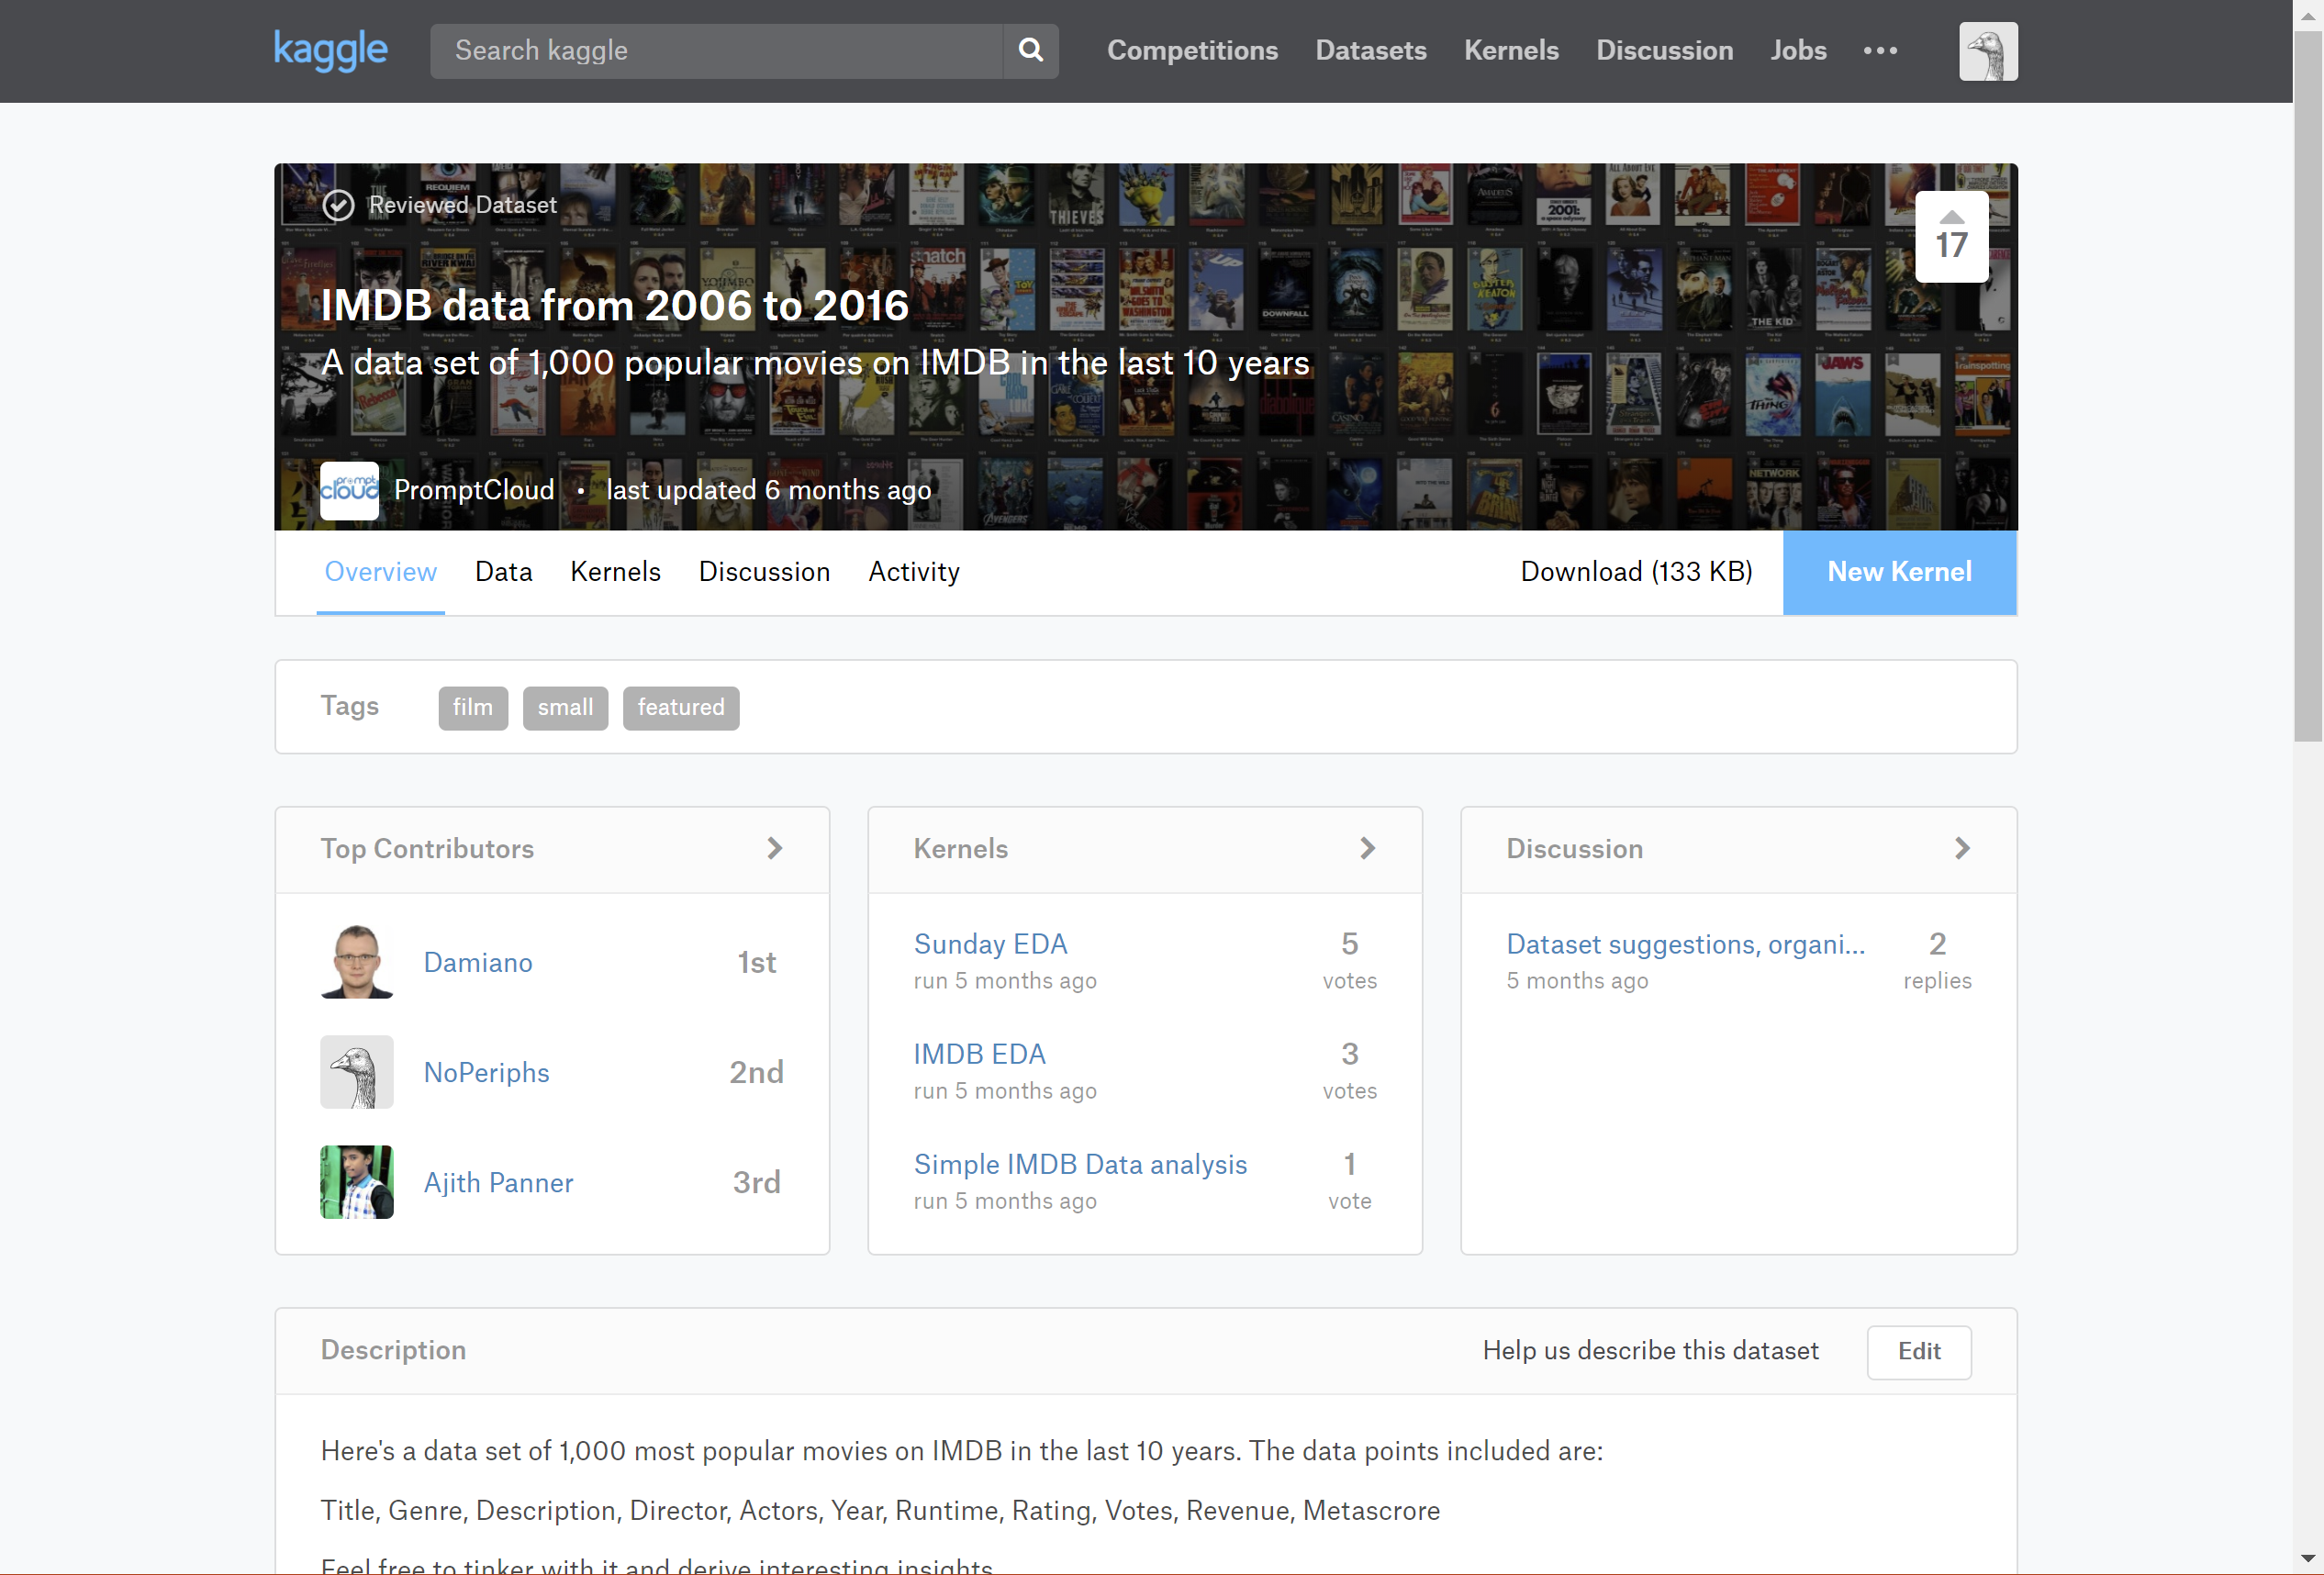
\includegraphics{kaggle-data.png}
  \subsection{IMDb}
  IMDb, formerly known as Internet Movie Database, is an online database
  of information related to films, television programs and video games,
  including cast, production crew, fictional characters, biographies,
  plot summaries, trivia and reviews, operated by IMDb.com, Inc., a
  subsidiary of Amazon.{[}Wikipedia{]}
  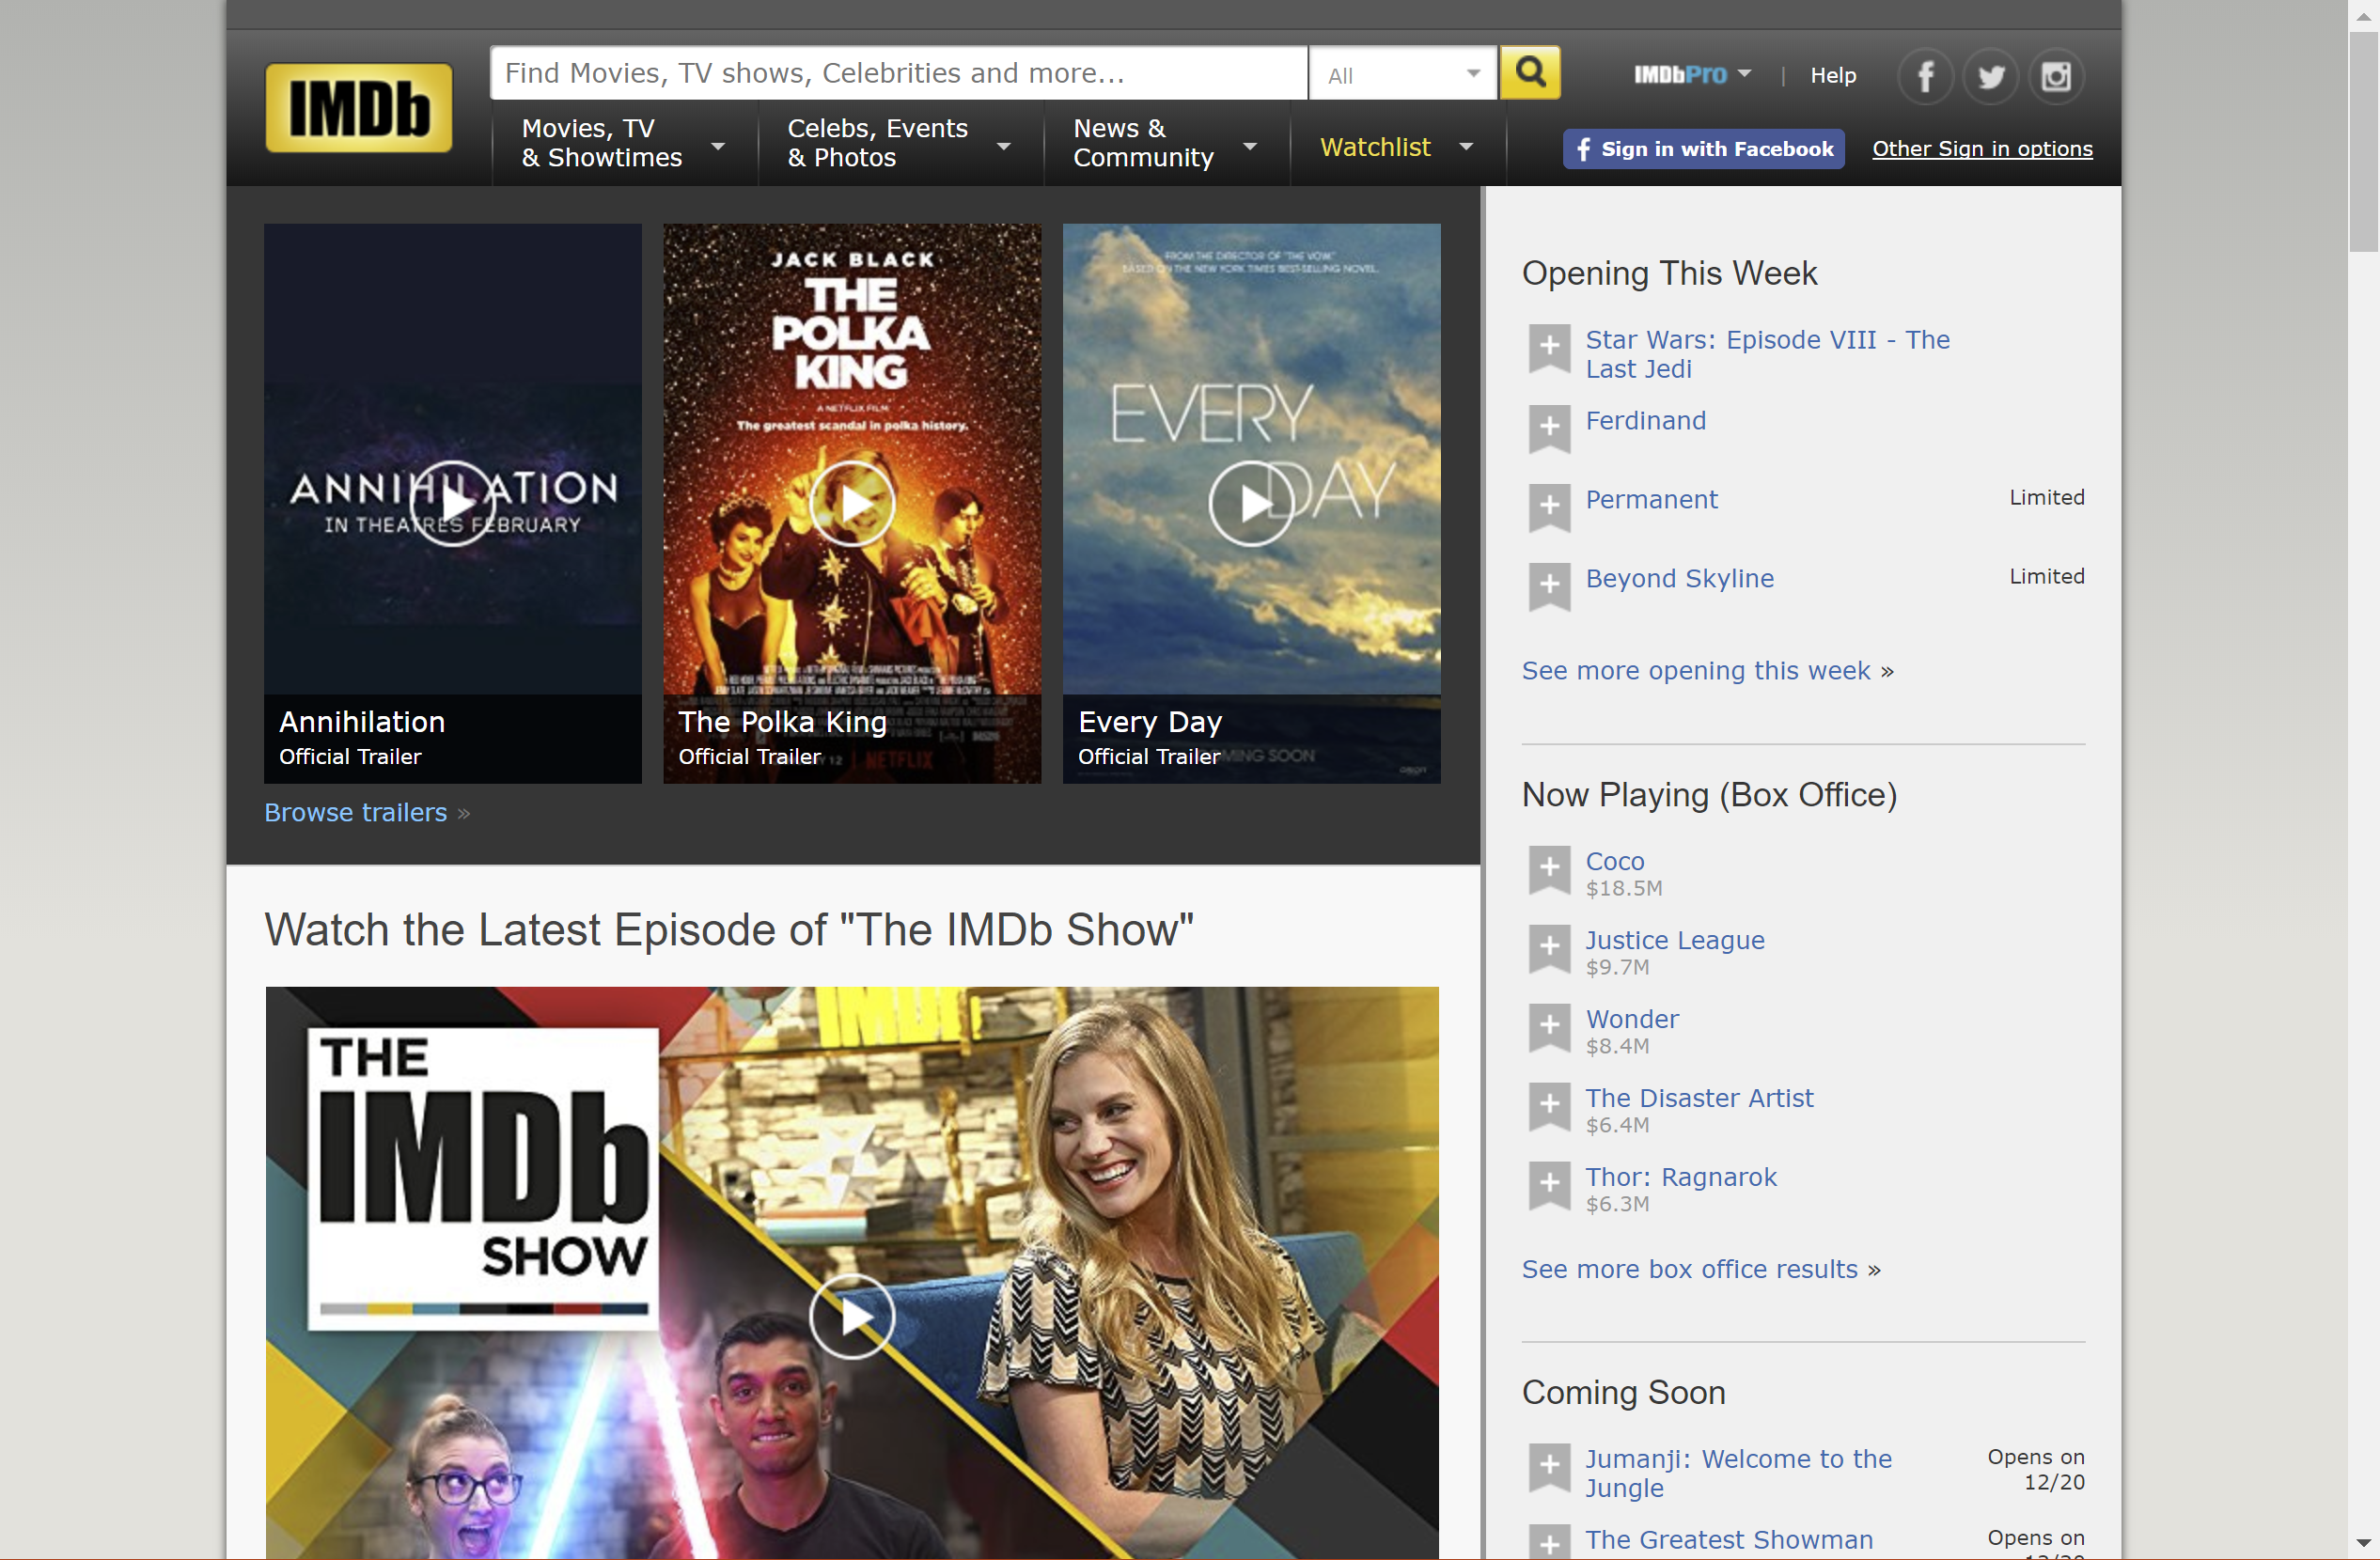
\includegraphics{imdb-mainpage.png}
  \subsubsection{Movies on IMDb}
  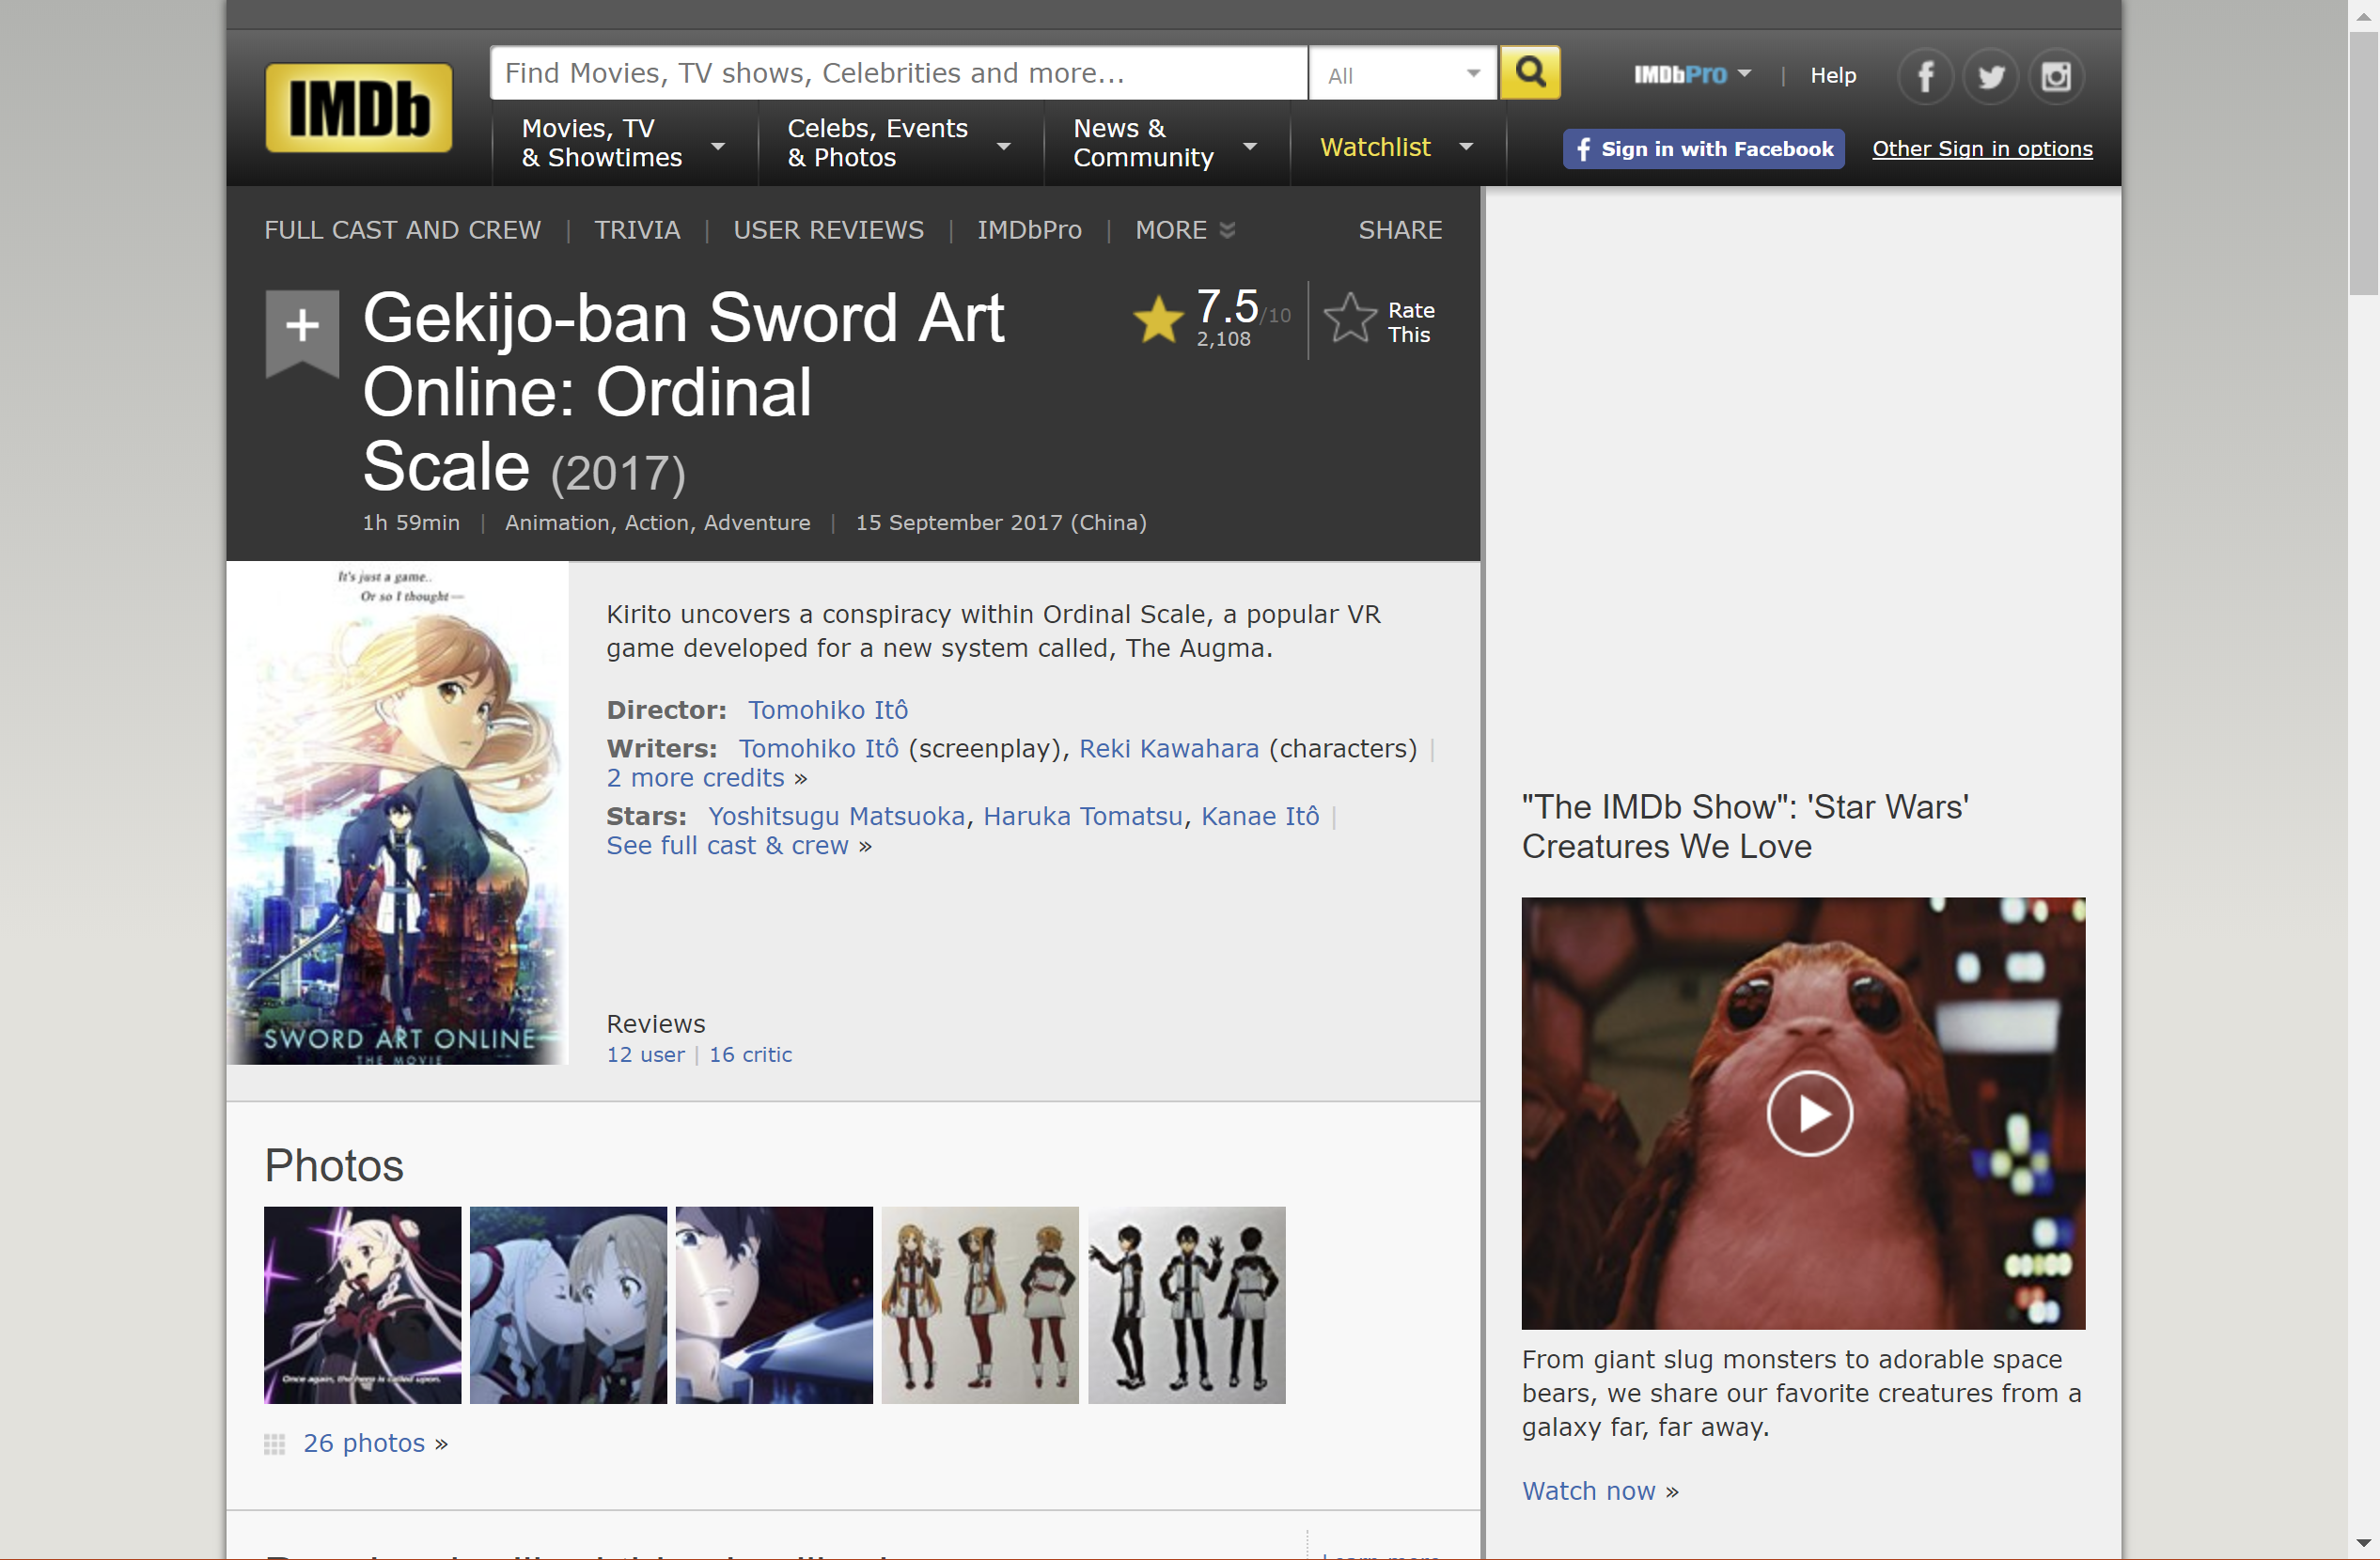
\includegraphics{imdb-movie.png}


    \section{Analyses}\label{analyses}

Five analyses were brought out by members in the group. 
\begin{itemize}
    \item Directors and Revenue \textbf{by Junru (Bill) Zhong}
    \item Directors and Rating \textbf{by Kefu (Frank) Wu}
    \item Genres and Time \textbf{by Yongsheng (Jeff) Fu}
    \item Rating and Metascore \textbf{by Kedun (Covey) Liu}
    \item Keywords in Films \textbf{by Jiaqi (Garfield) Wu}
\end{itemize}

\subsection{Analysis on Directors}\label{analysis-on-directors}

This analysis was posted by \textbf{Junru (Bill) Zhong}, and the
following aims were setted. 
\begin{itemize}
    \item Find out which director earned most.
    \item Find out the genres of the works of the five-most earned directors.
    \item Estimate how much each of them will get in their next film.
\end{itemize}
This analysis was brought by Python with package: pandas

    \begin{Verbatim}[commandchars=\\\{\}]
{\color{incolor}In [{\color{incolor}1}]:} \PY{c+c1}{\PYZsh{} Import package}
        \PY{k+kn}{import} \PY{n+nn}{pandas} \PY{k}{as} \PY{n+nn}{pd}
        \PY{c+c1}{\PYZsh{} Read data}
        \PY{n}{df} \PY{o}{=} \PY{n}{pd}\PY{o}{.}\PY{n}{read\PYZus{}csv}\PY{p}{(}\PY{l+s+s1}{\PYZsq{}}\PY{l+s+s1}{../Dataset/IMDB\PYZhy{}Movie\PYZhy{}Data.csv}\PY{l+s+s1}{\PYZsq{}}\PY{p}{)}
        \PY{n+nb}{print}\PY{p}{(}\PY{n}{df}\PY{o}{.}\PY{n}{head}\PY{p}{(}\PY{p}{)}\PY{p}{)}
\end{Verbatim}


    \begin{Verbatim}[commandchars=\\\{\}]
   Rank                    Title                     Genre  \textbackslash{}
0     1  Guardians of the Galaxy   Action,Adventure,Sci-Fi   
1     2               Prometheus  Adventure,Mystery,Sci-Fi   
2     3                    Split           Horror,Thriller   
3     4                     Sing   Animation,Comedy,Family   
4     5            Suicide Squad  Action,Adventure,Fantasy   

                                         Description              Director  \textbackslash{}
0  A group of intergalactic criminals are forced {\ldots}            James Gunn   
1  Following clues to the origin of mankind, a te{\ldots}          Ridley Scott   
2  Three girls are kidnapped by a man with a diag{\ldots}    M. Night Shyamalan   
3  In a city of humanoid animals, a hustling thea{\ldots}  Christophe Lourdelet   
4  A secret government agency recruits some of th{\ldots}            David Ayer   

                                              Actors  Year  Runtime (Minutes)  \textbackslash{}
0  Chris Pratt, Vin Diesel, Bradley Cooper, Zoe S{\ldots}  2014                121   
1  Noomi Rapace, Logan Marshall-Green, Michael Fa{\ldots}  2012                124   
2  James McAvoy, Anya Taylor-Joy, Haley Lu Richar{\ldots}  2016                117   
3  Matthew McConaughey,Reese Witherspoon, Seth Ma{\ldots}  2016                108   
4  Will Smith, Jared Leto, Margot Robbie, Viola D{\ldots}  2016                123   

   Rating   Votes  Revenue (Millions)  Metascore  
0     8.1  757074              333.13       76.0  
1     7.0  485820              126.46       65.0  
2     7.3  157606              138.12       62.0  
3     7.2   60545              270.32       59.0  
4     6.2  393727              325.02       40.0  

    \end{Verbatim}

    \subsubsection{Arranging Data}\label{arranging-data}

\begin{itemize}
\tightlist
\item
  Use \texttt{groupby} method provided by pandas, select all directors
  and their films' revenue.
\item
  Collect this data with the film count and total revenue of their
  works.
\item
  Drop the data with value of null.
\end{itemize}

    \begin{Verbatim}[commandchars=\\\{\}]
{\color{incolor}In [{\color{incolor}4}]:} \PY{c+c1}{\PYZsh{} List all directors.}
        \PY{n}{directorList} \PY{o}{=} \PY{n}{df}\PY{o}{.}\PY{n}{groupby}\PY{p}{(}\PY{l+s+s1}{\PYZsq{}}\PY{l+s+s1}{Director}\PY{l+s+s1}{\PYZsq{}}\PY{p}{)}\PY{p}{[}\PY{l+s+s1}{\PYZsq{}}\PY{l+s+s1}{Revenue (Millions)}\PY{l+s+s1}{\PYZsq{}}\PY{p}{]}\PY{o}{.}\PY{n}{agg}\PY{p}{(}\PY{p}{[}\PY{l+s+s1}{\PYZsq{}}\PY{l+s+s1}{sum}\PY{l+s+s1}{\PYZsq{}}\PY{p}{,} \PY{l+s+s1}{\PYZsq{}}\PY{l+s+s1}{count}\PY{l+s+s1}{\PYZsq{}}\PY{p}{]}\PY{p}{)}\PY{o}{.}\PY{n}{reset\PYZus{}index}\PY{p}{(}\PY{p}{)}
        \PY{c+c1}{\PYZsh{} Delete invalid data}
        \PY{n}{directorList} \PY{o}{=} \PY{n}{directorList}\PY{o}{.}\PY{n}{dropna}\PY{p}{(}\PY{p}{)}
        \PY{c+c1}{\PYZsh{} Print out result}
        \PY{n+nb}{print}\PY{p}{(}\PY{n}{directorList}\PY{o}{.}\PY{n}{head}\PY{p}{(}\PY{p}{)}\PY{p}{)}
\end{Verbatim}


    \begin{Verbatim}[commandchars=\\\{\}]
              Director     sum  count
0           Aamir Khan    1.20      1
1  Abdellatif Kechiche    2.20      1
3           Adam McKay  438.14      4
4        Adam Shankman  157.33      2
5         Adam Wingard   21.07      2

    \end{Verbatim}

    \subsubsection{Sort Data}\label{sort-data}

Sort the data according to the \textbf{average revenue} of each film
that the directors directed. 
\begin{itemize}
    \item Calculate the average revenue.
    \item Sort the list.
    \item Save the first five directors.
\end{itemize}

    \begin{Verbatim}[commandchars=\\\{\}]
{\color{incolor}In [{\color{incolor}6}]:} \PY{c+c1}{\PYZsh{} Get average revenue of each director.}
        \PY{n}{directorList}\PY{p}{[}\PY{l+s+s1}{\PYZsq{}}\PY{l+s+s1}{avg}\PY{l+s+s1}{\PYZsq{}}\PY{p}{]} \PY{o}{=} \PY{n}{directorList}\PY{p}{[}\PY{l+s+s1}{\PYZsq{}}\PY{l+s+s1}{sum}\PY{l+s+s1}{\PYZsq{}}\PY{p}{]} \PY{o}{/} \PY{n}{directorList}\PY{p}{[}\PY{l+s+s1}{\PYZsq{}}\PY{l+s+s1}{count}\PY{l+s+s1}{\PYZsq{}}\PY{p}{]}
        \PY{n+nb}{print}\PY{p}{(}\PY{n}{directorList}\PY{o}{.}\PY{n}{head}\PY{p}{(}\PY{p}{)}\PY{p}{)}
\end{Verbatim}


    \begin{Verbatim}[commandchars=\\\{\}]
              Director     sum  count      avg
0           Aamir Khan    1.20      1    1.200
1  Abdellatif Kechiche    2.20      1    2.200
3           Adam McKay  438.14      4  109.535
4        Adam Shankman  157.33      2   78.665
5         Adam Wingard   21.07      2   10.535

    \end{Verbatim}

    \begin{Verbatim}[commandchars=\\\{\}]
{\color{incolor}In [{\color{incolor}7}]:} \PY{c+c1}{\PYZsh{} Sorting by revenue, list the first five data.}
        \PY{n}{firstFive} \PY{o}{=} \PY{n}{directorList}\PY{o}{.}\PY{n}{sort\PYZus{}values}\PY{p}{(}\PY{l+s+s1}{\PYZsq{}}\PY{l+s+s1}{avg}\PY{l+s+s1}{\PYZsq{}}\PY{p}{,} \PY{n}{ascending}\PY{o}{=}\PY{k+kc}{False}\PY{p}{)}\PY{o}{.}\PY{n}{head}\PY{p}{(}\PY{p}{)}
        \PY{n+nb}{print}\PY{p}{(}\PY{n}{firstFive}\PY{p}{)}
\end{Verbatim}


    \begin{Verbatim}[commandchars=\\\{\}]
            Director      sum  count      avg
261    James Cameron   760.51      1  760.510
114  Colin Trevorrow   652.18      1  652.180
341      Joss Whedon  1082.27      2  541.135
377      Lee Unkrich   414.98      1  414.980
208        Gary Ross   408.00      1  408.000

    \end{Verbatim}

    \subsubsection{Genres of Directors'
Work}\label{genres-of-directors-work}

Go back to the original dataset, then match all entries of these
directors.

    \begin{Verbatim}[commandchars=\\\{\}]
{\color{incolor}In [{\color{incolor}8}]:} \PY{c+c1}{\PYZsh{} Searching their works.}
        \PY{n}{directorNames} \PY{o}{=} \PY{n}{firstFive}\PY{p}{[}\PY{l+s+s1}{\PYZsq{}}\PY{l+s+s1}{Director}\PY{l+s+s1}{\PYZsq{}}\PY{p}{]}
        \PY{k}{for} \PY{n}{directorName} \PY{o+ow}{in} \PY{n}{directorNames}\PY{p}{:}
            \PY{k}{for} \PY{n}{index}\PY{p}{,} \PY{n}{row} \PY{o+ow}{in} \PY{n}{df}\PY{o}{.}\PY{n}{iterrows}\PY{p}{(}\PY{p}{)}\PY{p}{:}
                \PY{k}{if} \PY{n}{row}\PY{p}{[}\PY{l+s+s1}{\PYZsq{}}\PY{l+s+s1}{Director}\PY{l+s+s1}{\PYZsq{}}\PY{p}{]} \PY{o}{==} \PY{n}{directorName}\PY{p}{:}
                    \PY{n+nb}{print}\PY{p}{(}\PY{n}{row}\PY{p}{[}\PY{l+s+s1}{\PYZsq{}}\PY{l+s+s1}{Director}\PY{l+s+s1}{\PYZsq{}}\PY{p}{]} \PY{o}{+} \PY{l+s+s1}{\PYZsq{}}\PY{l+s+s1}{, }\PY{l+s+s1}{\PYZsq{}} \PY{o}{+} \PY{n}{row}\PY{p}{[}\PY{l+s+s1}{\PYZsq{}}\PY{l+s+s1}{Genre}\PY{l+s+s1}{\PYZsq{}}\PY{p}{]} \PY{o}{+} \PY{l+s+s1}{\PYZsq{}}\PY{l+s+s1}{, }\PY{l+s+s1}{\PYZsq{}} \PY{o}{+} \PY{n}{row}\PY{p}{[}\PY{l+s+s1}{\PYZsq{}}\PY{l+s+s1}{Title}\PY{l+s+s1}{\PYZsq{}}\PY{p}{]}\PY{p}{)}
\end{Verbatim}


    \begin{Verbatim}[commandchars=\\\{\}]
James Cameron, Action,Adventure,Fantasy, Avatar
Colin Trevorrow, Action,Adventure,Sci-Fi, Jurassic World
Joss Whedon, Action,Sci-Fi, The Avengers
Joss Whedon, Action,Adventure,Sci-Fi, Avengers: Age of Ultron
Lee Unkrich, Animation,Adventure,Comedy, Toy Story 3
Gary Ross, Adventure,Sci-Fi,Thriller, The Hunger Games
Gary Ross, Action,Biography,Drama, Free State of Jones

    \end{Verbatim}

    \emph{One movie from \textbf{Gary Ross} was not calculated because there
is no revenue data.}

    \subsubsection{Summary}\label{summary}

\begin{itemize}
\tightlist
\item
  In the first five directors, seven of their works were recorded.
\item
  Six of seven films have the genre of \textbf{Action}, that means
  action films are popular.
\item
  Four of seven films have the genre of \textbf{Sci-Fi}, this
  genre is also popular.
\end{itemize}

    \subsection{Analysis on Directors by Rating}\label{analysis-on-directors-by-rating}

This analysis was posted by \textbf{Kefu (Frank) Wu}, and the following
aims were setted. 
\begin{itemize}
    \item Find out which director is praised most.
    \item Find out the genres of the works of the five-most praised directors.
    \item Estimate the rating that new film may get according to the genres of the film and its director.
\end{itemize}
This analysis was brought by Python with package: pandas

    \begin{Verbatim}[commandchars=\\\{\}]
{\color{incolor}In [{\color{incolor}3}]:} \PY{c+c1}{\PYZsh{} Show origin data}
        \PY{n+nb}{print}\PY{p}{(}\PY{n}{df}\PY{o}{.}\PY{n}{head}\PY{p}{(}\PY{p}{)}\PY{p}{)}
\end{Verbatim}


    \begin{Verbatim}[commandchars=\\\{\}]
   Rank                    Title                     Genre  \textbackslash{}
0     1  Guardians of the Galaxy   Action,Adventure,Sci-Fi   
1     2               Prometheus  Adventure,Mystery,Sci-Fi   
2     3                    Split           Horror,Thriller   
3     4                     Sing   Animation,Comedy,Family   
4     5            Suicide Squad  Action,Adventure,Fantasy   

                                         Description              Director  \textbackslash{}
0  A group of intergalactic criminals are forced {\ldots}            James Gunn   
1  Following clues to the origin of mankind, a te{\ldots}          Ridley Scott   
2  Three girls are kidnapped by a man with a diag{\ldots}    M. Night Shyamalan   
3  In a city of humanoid animals, a hustling thea{\ldots}  Christophe Lourdelet   
4  A secret government agency recruits some of th{\ldots}            David Ayer   

                                              Actors  Year  Runtime (Minutes)  \textbackslash{}
0  Chris Pratt, Vin Diesel, Bradley Cooper, Zoe S{\ldots}  2014                121   
1  Noomi Rapace, Logan Marshall-Green, Michael Fa{\ldots}  2012                124   
2  James McAvoy, Anya Taylor-Joy, Haley Lu Richar{\ldots}  2016                117   
3  Matthew McConaughey,Reese Witherspoon, Seth Ma{\ldots}  2016                108   
4  Will Smith, Jared Leto, Margot Robbie, Viola D{\ldots}  2016                123   

   Rating   Votes  Revenue (Millions)  Metascore  
0     8.1  757074              333.13       76.0  
1     7.0  485820              126.46       65.0  
2     7.3  157606              138.12       62.0  
3     7.2   60545              270.32       59.0  
4     6.2  393727              325.02       40.0  

    \end{Verbatim}

    \subsubsection{Arranging Data}\label{arranging-data}

\begin{itemize}
\tightlist
\item
  Use \texttt{groupby} method provided by pandas, select all directors
  and their films' rating.
\item
  Collect this data with the film count and sum up the rating of their
  works.
\end{itemize}

    \begin{Verbatim}[commandchars=\\\{\}]
{\color{incolor}In [{\color{incolor}4}]:} \PY{c+c1}{\PYZsh{} List all directors.}
        \PY{n}{directorList} \PY{o}{=} \PY{n}{df}\PY{o}{.}\PY{n}{groupby}\PY{p}{(}\PY{l+s+s1}{\PYZsq{}}\PY{l+s+s1}{Director}\PY{l+s+s1}{\PYZsq{}}\PY{p}{)}\PY{p}{[}\PY{l+s+s1}{\PYZsq{}}\PY{l+s+s1}{Rating}\PY{l+s+s1}{\PYZsq{}}\PY{p}{]}\PY{o}{.}\PY{n}{agg}\PY{p}{(}\PY{p}{[}\PY{l+s+s1}{\PYZsq{}}\PY{l+s+s1}{sum}\PY{l+s+s1}{\PYZsq{}}\PY{p}{,} \PY{l+s+s1}{\PYZsq{}}\PY{l+s+s1}{count}\PY{l+s+s1}{\PYZsq{}}\PY{p}{]}\PY{p}{)}\PY{o}{.}\PY{n}{reset\PYZus{}index}\PY{p}{(}\PY{p}{)}
        \PY{c+c1}{\PYZsh{} Print out result}
        \PY{n+nb}{print}\PY{p}{(}\PY{n}{directorList}\PY{o}{.}\PY{n}{head}\PY{p}{(}\PY{p}{)}\PY{p}{)}
\end{Verbatim}


    \begin{Verbatim}[commandchars=\\\{\}]
              Director   sum  count
0           Aamir Khan   8.5      1
1  Abdellatif Kechiche   7.8      1
2            Adam Leon   6.5      1
3           Adam McKay  28.0      4
4        Adam Shankman  12.6      2

    \end{Verbatim}

    \subsubsection{Sort Data}\label{sort-data}

Sort the data according to the \textbf{average rating} of each film that
the directors directed. * Calculate the average rating. * Sort the list.
* Save the top five directors that customers praised.

    \begin{Verbatim}[commandchars=\\\{\}]
{\color{incolor}In [{\color{incolor}5}]:} \PY{c+c1}{\PYZsh{} Get average rating of each director.}
        \PY{n}{directorList}\PY{p}{[}\PY{l+s+s1}{\PYZsq{}}\PY{l+s+s1}{avg}\PY{l+s+s1}{\PYZsq{}}\PY{p}{]} \PY{o}{=} \PY{n}{directorList}\PY{p}{[}\PY{l+s+s1}{\PYZsq{}}\PY{l+s+s1}{sum}\PY{l+s+s1}{\PYZsq{}}\PY{p}{]} \PY{o}{/} \PY{n}{directorList}\PY{p}{[}\PY{l+s+s1}{\PYZsq{}}\PY{l+s+s1}{count}\PY{l+s+s1}{\PYZsq{}}\PY{p}{]}
        \PY{n+nb}{print}\PY{p}{(}\PY{n}{directorList}\PY{o}{.}\PY{n}{head}\PY{p}{(}\PY{p}{)}\PY{p}{)}
\end{Verbatim}


    \begin{Verbatim}[commandchars=\\\{\}]
              Director   sum  count  avg
0           Aamir Khan   8.5      1  8.5
1  Abdellatif Kechiche   7.8      1  7.8
2            Adam Leon   6.5      1  6.5
3           Adam McKay  28.0      4  7.0
4        Adam Shankman  12.6      2  6.3

    \end{Verbatim}

    \begin{Verbatim}[commandchars=\\\{\}]
{\color{incolor}In [{\color{incolor}6}]:} \PY{c+c1}{\PYZsh{} Sorting by rating, list the first five data.}
        \PY{n}{firstFive} \PY{o}{=} \PY{n}{directorList}\PY{o}{.}\PY{n}{sort\PYZus{}values}\PY{p}{(}\PY{l+s+s1}{\PYZsq{}}\PY{l+s+s1}{avg}\PY{l+s+s1}{\PYZsq{}}\PY{p}{,} \PY{n}{ascending}\PY{o}{=}\PY{k+kc}{False}\PY{p}{)}\PY{o}{.}\PY{n}{head}\PY{p}{(}\PY{p}{)}
        \PY{n+nb}{print}\PY{p}{(}\PY{n}{firstFive}\PY{p}{)}
\end{Verbatim}


    \begin{Verbatim}[commandchars=\\\{\}]
                             Director   sum  count   avg
465                     Nitesh Tiwari   8.8      1  8.80
108                 Christopher Nolan  43.4      5  8.68
392                    Makoto Shinkai   8.6      1  8.60
470                   Olivier Nakache   8.6      1  8.60
194  Florian Henckel von Donnersmarck   8.5      1  8.50

    \end{Verbatim}

    \subsubsection{Genres of Directors'
Work}\label{genres-of-directors-work}

Go back to the original dataset, then match all entries of these
directors.

    \begin{Verbatim}[commandchars=\\\{\}]
{\color{incolor}In [{\color{incolor}23}]:} \PY{c+c1}{\PYZsh{} Searching their works.}
         \PY{n}{directorNames} \PY{o}{=} \PY{n}{firstFive}\PY{p}{[}\PY{l+s+s1}{\PYZsq{}}\PY{l+s+s1}{Director}\PY{l+s+s1}{\PYZsq{}}\PY{p}{]}
         \PY{k}{for} \PY{n}{directorName} \PY{o+ow}{in} \PY{n}{directorNames}\PY{p}{:}
             \PY{k}{for} \PY{n}{index}\PY{p}{,} \PY{n}{row} \PY{o+ow}{in} \PY{n}{df}\PY{o}{.}\PY{n}{iterrows}\PY{p}{(}\PY{p}{)}\PY{p}{:}
                 \PY{k}{if} \PY{n}{row}\PY{p}{[}\PY{l+s+s1}{\PYZsq{}}\PY{l+s+s1}{Director}\PY{l+s+s1}{\PYZsq{}}\PY{p}{]} \PY{o}{==} \PY{n}{directorName}\PY{p}{:}
                     \PY{n+nb}{print}\PY{p}{(}\PY{n}{row}\PY{p}{[}\PY{l+s+s1}{\PYZsq{}}\PY{l+s+s1}{Director}\PY{l+s+s1}{\PYZsq{}}\PY{p}{]} \PY{o}{+} \PY{l+s+s1}{\PYZsq{}}\PY{l+s+s1}{: }\PY{l+s+se}{\PYZbs{}n}\PY{l+s+se}{\PYZbs{}t}\PY{l+s+s1}{\PYZsq{}} \PY{o}{+} \PY{n}{row}\PY{p}{[}\PY{l+s+s1}{\PYZsq{}}\PY{l+s+s1}{Genre}\PY{l+s+s1}{\PYZsq{}}\PY{p}{]} \PY{o}{+} \PY{l+s+s1}{\PYZsq{}}\PY{l+s+s1}{, }\PY{l+s+s1}{\PYZsq{}} \PY{o}{+} \PY{n}{row}\PY{p}{[}\PY{l+s+s1}{\PYZsq{}}\PY{l+s+s1}{Title}\PY{l+s+s1}{\PYZsq{}}\PY{p}{]}\PY{p}{)}
\end{Verbatim}


    \begin{Verbatim}[commandchars=\\\{\}]
Nitesh Tiwari: 
	Action,Biography,Drama, Dangal
Christopher Nolan: 
	Adventure,Drama,Sci-Fi, Interstellar
Christopher Nolan: 
	Action,Crime,Drama, The Dark Knight
Christopher Nolan: 
	Drama,Mystery,Sci-Fi, The Prestige
Christopher Nolan: 
	Action,Adventure,Sci-Fi, Inception
Christopher Nolan: 
	Action,Thriller, The Dark Knight Rises
Makoto Shinkai: 
	Animation,Drama,Fantasy, Kimi no na wa
Olivier Nakache: 
	Biography,Comedy,Drama, The Intouchables
Florian Henckel von Donnersmarck: 
	Drama,Thriller, The Lives of Others

    \end{Verbatim}

    \subsubsection{Summary}\label{summary}

\begin{itemize}
\tightlist
\item
  We find out five director that are favored by their audience.
\item
  In the first five directors, nine of their works were recorded.
\item
  Among the directors, Chrostopher Nolan is the only director that can
  maintain high average rating after producing more than one film.
\item
  In Nolan's five works, there are three of them are action/sci-Fi,
  which means that Nolan is good at directoring action/sci-Fi film.
\end{itemize}

    \subsection{Genre's Analysis}\label{genres-analysis}

The fellowing python code analyze the revenue of each kind of moive in
past ten years. We can easily learn what kind of moive is easiest to make money.

    \begin{Verbatim}[commandchars=\\\{\}]
{\color{incolor}In [{\color{incolor}1}]:} \PY{c+c1}{\PYZsh{}Import packages}
        
        \PY{k+kn}{import} \PY{n+nn}{numpy} \PY{k}{as} \PY{n+nn}{np}
        \PY{k+kn}{import} \PY{n+nn}{matplotlib}\PY{n+nn}{.}\PY{n+nn}{pyplot} \PY{k}{as} \PY{n+nn}{plt}
        \PY{o}{\PYZpc{}}\PY{k}{matplotlib} inline
        \PY{k+kn}{import} \PY{n+nn}{pandas} \PY{k}{as} \PY{n+nn}{pd}
        \PY{k+kn}{import} \PY{n+nn}{seaborn} \PY{k}{as} \PY{n+nn}{sns}
        \PY{n}{sns}\PY{o}{.}\PY{n}{set}\PY{p}{(}\PY{n}{style}\PY{o}{=}\PY{l+s+s1}{\PYZsq{}}\PY{l+s+s1}{white}\PY{l+s+s1}{\PYZsq{}}\PY{p}{,} \PY{n}{color\PYZus{}codes}\PY{o}{=}\PY{k+kc}{True}\PY{p}{,} \PY{n}{font\PYZus{}scale}\PY{o}{=}\PY{l+m+mf}{1.25}\PY{p}{)}
        \PY{k+kn}{import} \PY{n+nn}{itertools}
\end{Verbatim}


    \subsubsection{Load Dataset}\label{load-dataset}

First, we read the IMDB dataset csv file, and load it in to a DataFrame.
Here are the first 5 row of the dataset.

    \begin{Verbatim}[commandchars=\\\{\}]
{\color{incolor}In [{\color{incolor}2}]:} \PY{c+c1}{\PYZsh{}Import the data into a DF and view the first 5 entries}
        
        \PY{n}{imdb} \PY{o}{=} \PY{n}{pd}\PY{o}{.}\PY{n}{read\PYZus{}csv}\PY{p}{(}\PY{l+s+s1}{\PYZsq{}}\PY{l+s+s1}{../Dataset/IMDB\PYZhy{}Movie\PYZhy{}Data.csv}\PY{l+s+s1}{\PYZsq{}}\PY{p}{)}
        \PY{n}{imdb}\PY{o}{.}\PY{n}{head}\PY{p}{(}\PY{p}{)}
\end{Verbatim}


\begin{Verbatim}[commandchars=\\\{\}]
{\color{outcolor}Out[{\color{outcolor}2}]:}    Rank                    Title                     Genre  \textbackslash{}
        0     1  Guardians of the Galaxy   Action,Adventure,Sci-Fi   
        1     2               Prometheus  Adventure,Mystery,Sci-Fi   
        2     3                    Split           Horror,Thriller   
        3     4                     Sing   Animation,Comedy,Family   
        4     5            Suicide Squad  Action,Adventure,Fantasy   
        
                                                 Description              Director  \textbackslash{}
        0  A group of intergalactic criminals are forced {\ldots}            James Gunn   
        1  Following clues to the origin of mankind, a te{\ldots}          Ridley Scott   
        2  Three girls are kidnapped by a man with a diag{\ldots}    M. Night Shyamalan   
        3  In a city of humanoid animals, a hustling thea{\ldots}  Christophe Lourdelet   
        4  A secret government agency recruits some of th{\ldots}            David Ayer   
        
                                                      Actors  Year  Runtime (Minutes)  \textbackslash{}
        0  Chris Pratt, Vin Diesel, Bradley Cooper, Zoe S{\ldots}  2014                121   
        1  Noomi Rapace, Logan Marshall-Green, Michael Fa{\ldots}  2012                124   
        2  James McAvoy, Anya Taylor-Joy, Haley Lu Richar{\ldots}  2016                117   
        3  Matthew McConaughey,Reese Witherspoon, Seth Ma{\ldots}  2016                108   
        4  Will Smith, Jared Leto, Margot Robbie, Viola D{\ldots}  2016                123   
        
           Rating   Votes  Revenue (Millions)  Metascore  
        0     8.1  757074              333.13       76.0  
        1     7.0  485820              126.46       65.0  
        2     7.3  157606              138.12       62.0  
        3     7.2   60545              270.32       59.0  
        4     6.2  393727              325.02       40.0  
\end{Verbatim}
Now, we use above dataset to plot a scatter graph so that we can know the \textbf{distribution of moives and their revenue}

    \begin{Verbatim}[commandchars=\\\{\}]
{\color{incolor}In [{\color{incolor}3}]:} \PY{c+c1}{\PYZsh{}Plot the Revenue in recent ten years}
        \PY{n}{sns}\PY{o}{.}\PY{n}{jointplot}\PY{p}{(}\PY{n}{x}\PY{o}{=}\PY{l+s+s1}{\PYZsq{}}\PY{l+s+s1}{Year}\PY{l+s+s1}{\PYZsq{}}\PY{p}{,} \PY{n}{y}\PY{o}{=}\PY{l+s+s1}{\PYZsq{}}\PY{l+s+s1}{Revenue (Millions)}\PY{l+s+s1}{\PYZsq{}}\PY{p}{,} \PY{n}{data}\PY{o}{=}\PY{n}{imdb}\PY{p}{,} \PY{n}{alpha}\PY{o}{=}\PY{l+m+mf}{0.5}\PY{p}{,} \PY{n}{color}\PY{o}{=}\PY{l+s+s1}{\PYZsq{}}\PY{l+s+s1}{r}\PY{l+s+s1}{\PYZsq{}}\PY{p}{,} \PY{n}{size}\PY{o}{=}\PY{l+m+mi}{10}\PY{p}{,} \PY{n}{space}\PY{o}{=}\PY{l+m+mi}{0}\PY{p}{)}
\end{Verbatim}


\begin{Verbatim}[commandchars=\\\{\}]
{\color{outcolor}Out[{\color{outcolor}3}]:} <seaborn.axisgrid.JointGrid at 0x7fa0c64a0f98>
\end{Verbatim}
            
    \begin{center}
    \adjustimage{max size={0.9\linewidth}{0.9\paperheight}}{output_27_1.png}
    \end{center}
    { \hspace*{\fill} \\}
    
As the result shows, we know that more and more file are made in recent
year. Besides, the result also shows us that most moive's revenue is
less than 200 Millions dollor.

\subsubsection{Question}\label{question}
\begin{itemize}
    \item \textbf{What kind of moive are easiest to earn money?}
    \item \textbf{For answering this question, let's divde moive into different genre.}
\end{itemize}
By using unique() build-in function of pandas package. And record them
by iteration, finally we got 20 unique genres. Here are the result.

    \begin{Verbatim}[commandchars=\\\{\}]
{\color{incolor}In [{\color{incolor}4}]:} \PY{c+c1}{\PYZsh{}Get unique genres}
        
        \PY{n}{unique\PYZus{}genres} \PY{o}{=} \PY{n}{imdb}\PY{p}{[}\PY{l+s+s1}{\PYZsq{}}\PY{l+s+s1}{Genre}\PY{l+s+s1}{\PYZsq{}}\PY{p}{]}\PY{o}{.}\PY{n}{unique}\PY{p}{(}\PY{p}{)}
        \PY{n}{individual\PYZus{}genres} \PY{o}{=} \PY{p}{[}\PY{p}{]}
        \PY{k}{for} \PY{n}{genre} \PY{o+ow}{in} \PY{n}{unique\PYZus{}genres}\PY{p}{:}
            \PY{n}{individual\PYZus{}genres}\PY{o}{.}\PY{n}{append}\PY{p}{(}\PY{n}{genre}\PY{o}{.}\PY{n}{split}\PY{p}{(}\PY{l+s+s1}{\PYZsq{}}\PY{l+s+s1}{,}\PY{l+s+s1}{\PYZsq{}}\PY{p}{)}\PY{p}{)}
        \PY{n}{individual\PYZus{}genres} \PY{o}{=} \PY{n+nb}{list}\PY{p}{(}\PY{n}{itertools}\PY{o}{.}\PY{n}{chain}\PY{o}{.}\PY{n}{from\PYZus{}iterable}\PY{p}{(}\PY{n}{individual\PYZus{}genres}\PY{p}{)}\PY{p}{)}
        \PY{n}{individual\PYZus{}genres} \PY{o}{=} \PY{n+nb}{set}\PY{p}{(}\PY{n}{individual\PYZus{}genres}\PY{p}{)}
        \PY{n}{individual\PYZus{}genres}
\end{Verbatim}


\begin{Verbatim}[commandchars=\\\{\}]
{\color{outcolor}Out[{\color{outcolor}4}]:} \{'Action',
         'Adventure',
         'Animation',
         'Biography',
         'Comedy',
         'Crime',
         'Drama',
         'Family',
         'Fantasy',
         'History',
         'Horror',
         'Music',
         'Musical',
         'Mystery',
         'Romance',
         'Sci-Fi',
         'Sport',
         'Thriller',
         'War',
         'Western'\}
\end{Verbatim}
            
After we get each individual genres. We plot how many films of each genre were made by year onto a bar graph

    \begin{Verbatim}[commandchars=\\\{\}]
{\color{incolor}In [{\color{incolor}5}]:} \PY{c+c1}{\PYZsh{}Now we can iterate through each genre, counting the number of films that contain that genre}
        \PY{c+c1}{\PYZsh{}then plot how many films of each genre were made by year onto a bar graph}
        
        \PY{n+nb}{print}\PY{p}{(}\PY{l+s+s1}{\PYZsq{}}\PY{l+s+s1}{Number of movies in each genre: }\PY{l+s+se}{\PYZbs{}n}\PY{l+s+s1}{\PYZsq{}}\PY{p}{)}
        
        \PY{k}{for} \PY{n}{genre} \PY{o+ow}{in} \PY{n}{individual\PYZus{}genres}\PY{p}{:}
            \PY{n}{current\PYZus{}genre} \PY{o}{=} \PY{n}{imdb}\PY{p}{[}\PY{l+s+s1}{\PYZsq{}}\PY{l+s+s1}{Genre}\PY{l+s+s1}{\PYZsq{}}\PY{p}{]}\PY{o}{.}\PY{n}{str}\PY{o}{.}\PY{n}{contains}\PY{p}{(}\PY{n}{genre}\PY{p}{)}\PY{o}{.}\PY{n}{fillna}\PY{p}{(}\PY{k+kc}{False}\PY{p}{)}
            \PY{n}{plt}\PY{o}{.}\PY{n}{figure}\PY{p}{(}\PY{p}{)}
            \PY{n}{plt}\PY{o}{.}\PY{n}{xlabel}\PY{p}{(}\PY{l+s+s1}{\PYZsq{}}\PY{l+s+s1}{Year}\PY{l+s+s1}{\PYZsq{}}\PY{p}{)}
            \PY{n}{plt}\PY{o}{.}\PY{n}{ylabel}\PY{p}{(}\PY{l+s+s1}{\PYZsq{}}\PY{l+s+s1}{Number of Movies Made}\PY{l+s+s1}{\PYZsq{}}\PY{p}{)}
            \PY{n}{plt}\PY{o}{.}\PY{n}{title}\PY{p}{(}\PY{n+nb}{str}\PY{p}{(}\PY{n}{genre}\PY{p}{)}\PY{p}{)}
            \PY{n}{imdb}\PY{p}{[}\PY{n}{current\PYZus{}genre}\PY{p}{]}\PY{o}{.}\PY{n}{Year}\PY{o}{.}\PY{n}{value\PYZus{}counts}\PY{p}{(}\PY{p}{)}\PY{o}{.}\PY{n}{sort\PYZus{}index}\PY{p}{(}\PY{p}{)}\PY{o}{.}\PY{n}{plot}\PY{p}{(}\PY{n}{kind}\PY{o}{=}\PY{l+s+s1}{\PYZsq{}}\PY{l+s+s1}{bar}\PY{l+s+s1}{\PYZsq{}}\PY{p}{,} \PY{n}{color}\PY{o}{=}\PY{l+s+s1}{\PYZsq{}}\PY{l+s+s1}{r}\PY{l+s+s1}{\PYZsq{}}\PY{p}{,} \PY{n}{alpha}\PY{o}{=}\PY{l+m+mf}{0.5}\PY{p}{,} \PY{n}{rot}\PY{o}{=}\PY{l+m+mi}{45}\PY{p}{)}
            \PY{n+nb}{print}\PY{p}{(}\PY{n}{genre}\PY{p}{,} \PY{n+nb}{len}\PY{p}{(}\PY{n}{imdb}\PY{p}{[}\PY{n}{current\PYZus{}genre}\PY{p}{]}\PY{p}{)}\PY{p}{)}
\end{Verbatim}


    \begin{Verbatim}[commandchars=\\\{\}]
Number of movies in each genre: 

Music 21
Comedy 279
Romance 141
Action 303
Mystery 106
Family 51
Drama 513
Biography 81
Sci-Fi 120
History 29
Musical 5
Adventure 259
Thriller 195
Fantasy 101
War 13
Animation 49
Sport 18
Horror 119
Western 7
Crime 150

    \end{Verbatim}

    \begin{center}
    \adjustimage{max size={0.9\linewidth}{0.9\paperheight}}{output_31_1.png}
    \end{center}
    { \hspace*{\fill} \\}
    
    \begin{center}
    \adjustimage{max size={0.9\linewidth}{0.9\paperheight}}{output_31_2.png}
    \end{center}
    { \hspace*{\fill} \\}
    
    \begin{center}
    \adjustimage{max size={0.9\linewidth}{0.9\paperheight}}{output_31_3.png}
    \end{center}
    { \hspace*{\fill} \\}
    
    \begin{center}
    \adjustimage{max size={0.9\linewidth}{0.9\paperheight}}{output_31_4.png}
    \end{center}
    { \hspace*{\fill} \\}
    
    \begin{center}
    \adjustimage{max size={0.9\linewidth}{0.9\paperheight}}{output_31_5.png}
    \end{center}
    { \hspace*{\fill} \\}
    
    \begin{center}
    \adjustimage{max size={0.9\linewidth}{0.9\paperheight}}{output_31_6.png}
    \end{center}
    { \hspace*{\fill} \\}
    
    \begin{center}
    \adjustimage{max size={0.9\linewidth}{0.9\paperheight}}{output_31_7.png}
    \end{center}
    { \hspace*{\fill} \\}
    
    \begin{center}
    \adjustimage{max size={0.9\linewidth}{0.9\paperheight}}{output_31_8.png}
    \end{center}
    { \hspace*{\fill} \\}
    
    \begin{center}
    \adjustimage{max size={0.9\linewidth}{0.9\paperheight}}{output_31_9.png}
    \end{center}
    { \hspace*{\fill} \\}
    
    \begin{center}
    \adjustimage{max size={0.9\linewidth}{0.9\paperheight}}{output_31_10.png}
    \end{center}
    { \hspace*{\fill} \\}
    
    \begin{center}
    \adjustimage{max size={0.9\linewidth}{0.9\paperheight}}{output_31_11.png}
    \end{center}
    { \hspace*{\fill} \\}
    
    \begin{center}
    \adjustimage{max size={0.9\linewidth}{0.9\paperheight}}{output_31_12.png}
    \end{center}
    { \hspace*{\fill} \\}
    
    \begin{center}
    \adjustimage{max size={0.9\linewidth}{0.9\paperheight}}{output_31_13.png}
    \end{center}
    { \hspace*{\fill} \\}
    
    \begin{center}
    \adjustimage{max size={0.9\linewidth}{0.9\paperheight}}{output_31_14.png}
    \end{center}
    { \hspace*{\fill} \\}
    
    \begin{center}
    \adjustimage{max size={0.9\linewidth}{0.9\paperheight}}{output_31_15.png}
    \end{center}
    { \hspace*{\fill} \\}
    
    \begin{center}
    \adjustimage{max size={0.9\linewidth}{0.9\paperheight}}{output_31_16.png}
    \end{center}
    { \hspace*{\fill} \\}
    
    \begin{center}
    \adjustimage{max size={0.9\linewidth}{0.9\paperheight}}{output_31_17.png}
    \end{center}
    { \hspace*{\fill} \\}
    
    \begin{center}
    \adjustimage{max size={0.9\linewidth}{0.9\paperheight}}{output_31_18.png}
    \end{center}
    { \hspace*{\fill} \\}
    
    \begin{center}
    \adjustimage{max size={0.9\linewidth}{0.9\paperheight}}{output_31_19.png}
    \end{center}
    { \hspace*{\fill} \\}
    
    \begin{center}
    \adjustimage{max size={0.9\linewidth}{0.9\paperheight}}{output_31_20.png}
    \end{center}
    { \hspace*{\fill} \\}
    
    As all bar charts show above. Almost all kinds of moive trend to
increasing their production as time going.

\subsubsection{Question}\label{question}

\textbf{However, does it means all kinds of moive are become easier to
make money than before?}
\\
For answering this question, let's calculate the average revenue of
different kind of moives. And sort them by year to draw bar charts.

    \begin{Verbatim}[commandchars=\\\{\}]
{\color{incolor}In [{\color{incolor}6}]:} \PY{c+c1}{\PYZsh{}Count the average revenue of each genre of film by year}
        
        \PY{n}{year}\PY{o}{=}\PY{p}{\PYZob{}}\PY{l+s+s1}{\PYZsq{}}\PY{l+s+s1}{Year}\PY{l+s+s1}{\PYZsq{}}\PY{p}{:}\PY{p}{[}\PY{l+m+mi}{2006}\PY{p}{,}\PY{l+m+mi}{2007}\PY{p}{,}\PY{l+m+mi}{2008}\PY{p}{,}\PY{l+m+mi}{2009}\PY{p}{,}\PY{l+m+mi}{2010}\PY{p}{,}\PY{l+m+mi}{2011}\PY{p}{,}\PY{l+m+mi}{2012}\PY{p}{,}\PY{l+m+mi}{2013}\PY{p}{,}\PY{l+m+mi}{2014}\PY{p}{,}\PY{l+m+mi}{2015}\PY{p}{,}\PY{l+m+mi}{2016}\PY{p}{]}\PY{p}{\PYZcb{}}
        \PY{n}{YMR}\PY{o}{=}\PY{n}{pd}\PY{o}{.}\PY{n}{DataFrame}\PY{p}{(}\PY{n}{year}\PY{p}{)}
        \PY{k}{for} \PY{n}{genre} \PY{o+ow}{in} \PY{n}{individual\PYZus{}genres}\PY{p}{:}
            \PY{n}{current\PYZus{}genre} \PY{o}{=} \PY{n}{imdb}\PY{p}{[}\PY{l+s+s1}{\PYZsq{}}\PY{l+s+s1}{Genre}\PY{l+s+s1}{\PYZsq{}}\PY{p}{]}\PY{o}{.}\PY{n}{str}\PY{o}{.}\PY{n}{contains}\PY{p}{(}\PY{n}{genre}\PY{p}{)}\PY{o}{.}\PY{n}{fillna}\PY{p}{(}\PY{k+kc}{False}\PY{p}{)}
            \PY{n}{df} \PY{o}{=} \PY{n}{imdb}\PY{p}{[}\PY{n}{current\PYZus{}genre}\PY{p}{]}
            \PY{n}{genre\PYZus{}revenue}\PY{o}{=}\PY{n}{df}\PY{p}{[}\PY{p}{[}\PY{l+s+s1}{\PYZsq{}}\PY{l+s+s1}{Year}\PY{l+s+s1}{\PYZsq{}}\PY{p}{,}\PY{l+s+s1}{\PYZsq{}}\PY{l+s+s1}{Revenue (Millions)}\PY{l+s+s1}{\PYZsq{}}\PY{p}{]}\PY{p}{]}\PY{o}{.}\PY{n}{fillna}\PY{p}{(}\PY{l+m+mi}{0}\PY{p}{)} 
            \PY{n}{GR}\PY{o}{=}\PY{n}{genre\PYZus{}revenue}\PY{o}{.}\PY{n}{groupby}\PY{p}{(}\PY{l+s+s1}{\PYZsq{}}\PY{l+s+s1}{Year}\PY{l+s+s1}{\PYZsq{}}\PY{p}{)}\PY{p}{[}\PY{l+s+s1}{\PYZsq{}}\PY{l+s+s1}{Revenue (Millions)}\PY{l+s+s1}{\PYZsq{}}\PY{p}{]}\PY{o}{.}\PY{n}{agg}\PY{p}{(}\PY{p}{[}\PY{l+s+s1}{\PYZsq{}}\PY{l+s+s1}{sum}\PY{l+s+s1}{\PYZsq{}}\PY{p}{,}\PY{l+s+s1}{\PYZsq{}}\PY{l+s+s1}{count}\PY{l+s+s1}{\PYZsq{}}\PY{p}{]}\PY{p}{)}\PY{o}{.}\PY{n}{fillna}\PY{p}{(}\PY{l+m+mi}{0}\PY{p}{)} 
            \PY{n}{GR}\PY{p}{[}\PY{l+s+s1}{\PYZsq{}}\PY{l+s+s1}{Average Revenue (Millions)}\PY{l+s+s1}{\PYZsq{}}\PY{p}{]}\PY{o}{=}\PY{n}{GR}\PY{p}{[}\PY{l+s+s1}{\PYZsq{}}\PY{l+s+s1}{sum}\PY{l+s+s1}{\PYZsq{}}\PY{p}{]}\PY{o}{/}\PY{n}{GR}\PY{p}{[}\PY{l+s+s1}{\PYZsq{}}\PY{l+s+s1}{count}\PY{l+s+s1}{\PYZsq{}}\PY{p}{]}
            \PY{n}{GR}\PY{o}{.}\PY{n}{plot}\PY{p}{(}\PY{n}{y}\PY{o}{=}\PY{l+s+s1}{\PYZsq{}}\PY{l+s+s1}{Average Revenue (Millions)}\PY{l+s+s1}{\PYZsq{}}\PY{p}{,}\PY{n}{kind}\PY{o}{=}\PY{l+s+s1}{\PYZsq{}}\PY{l+s+s1}{bar}\PY{l+s+s1}{\PYZsq{}}\PY{p}{,} \PY{n}{color}\PY{o}{=}\PY{l+s+s1}{\PYZsq{}}\PY{l+s+s1}{b}\PY{l+s+s1}{\PYZsq{}}\PY{p}{,} \PY{n}{alpha}\PY{o}{=}\PY{l+m+mf}{0.5}\PY{p}{,} \PY{n}{rot}\PY{o}{=}\PY{l+m+mi}{45}\PY{p}{,}\PY{n}{title}\PY{o}{=}\PY{n}{genre}\PY{p}{)}
            \PY{n+nb}{sum} \PY{o}{=} \PY{n}{genre\PYZus{}revenue}\PY{p}{[}\PY{l+s+s1}{\PYZsq{}}\PY{l+s+s1}{Revenue (Millions)}\PY{l+s+s1}{\PYZsq{}}\PY{p}{]}\PY{o}{.}\PY{n}{sum}\PY{p}{(}\PY{p}{)}
            \PY{n}{count} \PY{o}{=} \PY{n+nb}{len}\PY{p}{(}\PY{n}{genre\PYZus{}revenue}\PY{p}{)}
            \PY{n}{AR}\PY{o}{=}\PY{n}{GR}\PY{p}{[}\PY{l+s+s1}{\PYZsq{}}\PY{l+s+s1}{Average Revenue (Millions)}\PY{l+s+s1}{\PYZsq{}}\PY{p}{]}\PY{o}{.}\PY{n}{values}
            \PY{k}{if} \PY{n+nb}{len}\PY{p}{(}\PY{n}{AR}\PY{p}{)} \PY{o}{==} \PY{l+m+mi}{11}\PY{p}{:}
                 \PY{n}{YMR}\PY{p}{[}\PY{n}{genre}\PY{p}{]}\PY{o}{=}\PY{p}{[}\PY{n}{AR}\PY{p}{[}\PY{l+m+mi}{0}\PY{p}{]}\PY{p}{,}\PY{n}{AR}\PY{p}{[}\PY{l+m+mi}{1}\PY{p}{]}\PY{p}{,}\PY{n}{AR}\PY{p}{[}\PY{l+m+mi}{2}\PY{p}{]}\PY{p}{,}\PY{n}{AR}\PY{p}{[}\PY{l+m+mi}{3}\PY{p}{]}\PY{p}{,}\PY{n}{AR}\PY{p}{[}\PY{l+m+mi}{4}\PY{p}{]}\PY{p}{,}\PY{n}{AR}\PY{p}{[}\PY{l+m+mi}{5}\PY{p}{]}\PY{p}{,}\PY{n}{AR}\PY{p}{[}\PY{l+m+mi}{6}\PY{p}{]}\PY{p}{,}\PY{n}{AR}\PY{p}{[}\PY{l+m+mi}{7}\PY{p}{]}\PY{p}{,}\PY{n}{AR}\PY{p}{[}\PY{l+m+mi}{8}\PY{p}{]}\PY{p}{,}\PY{n}{AR}\PY{p}{[}\PY{l+m+mi}{9}\PY{p}{]}\PY{p}{,}\PY{n}{AR}\PY{p}{[}\PY{l+m+mi}{10}\PY{p}{]}\PY{p}{]}
            \PY{k}{elif} \PY{n+nb}{len}\PY{p}{(}\PY{n}{AR}\PY{p}{)} \PY{o}{==} \PY{l+m+mi}{6}\PY{p}{:}
                \PY{n}{YMR}\PY{p}{[}\PY{n}{genre}\PY{p}{]}\PY{o}{=}\PY{p}{[}\PY{n}{np}\PY{o}{.}\PY{n}{nan}\PY{p}{,}\PY{n}{np}\PY{o}{.}\PY{n}{nan}\PY{p}{,}\PY{n}{np}\PY{o}{.}\PY{n}{nan}\PY{p}{,}\PY{n}{np}\PY{o}{.}\PY{n}{nan}\PY{p}{,}\PY{n}{AR}\PY{p}{[}\PY{l+m+mi}{0}\PY{p}{]}\PY{p}{,}\PY{n}{np}\PY{o}{.}\PY{n}{nan}\PY{p}{,}\PY{n}{AR}\PY{p}{[}\PY{l+m+mi}{1}\PY{p}{]}\PY{p}{,}\PY{n}{AR}\PY{p}{[}\PY{l+m+mi}{2}\PY{p}{]}\PY{p}{,}\PY{n}{AR}\PY{p}{[}\PY{l+m+mi}{3}\PY{p}{]}\PY{p}{,}\PY{n}{AR}\PY{p}{[}\PY{l+m+mi}{4}\PY{p}{]}\PY{p}{,}\PY{n}{AR}\PY{p}{[}\PY{l+m+mi}{5}\PY{p}{]}\PY{p}{]}
            \PY{k}{elif} \PY{n+nb}{len}\PY{p}{(}\PY{n}{AR}\PY{p}{)} \PY{o}{==}\PY{l+m+mi}{3}\PY{p}{:}
                \PY{n}{YMR}\PY{p}{[}\PY{n}{genre}\PY{p}{]}\PY{o}{=}\PY{p}{[}\PY{n}{np}\PY{o}{.}\PY{n}{nan}\PY{p}{,}\PY{n}{AR}\PY{p}{[}\PY{l+m+mi}{0}\PY{p}{]}\PY{p}{,}\PY{n}{AR}\PY{p}{[}\PY{l+m+mi}{1}\PY{p}{]}\PY{p}{,}\PY{n}{np}\PY{o}{.}\PY{n}{nan}\PY{p}{,}\PY{n}{np}\PY{o}{.}\PY{n}{nan}\PY{p}{,}\PY{n}{np}\PY{o}{.}\PY{n}{nan}\PY{p}{,}\PY{n}{AR}\PY{p}{[}\PY{l+m+mi}{2}\PY{p}{]}\PY{p}{,}\PY{n}{np}\PY{o}{.}\PY{n}{nan}\PY{p}{,}\PY{n}{np}\PY{o}{.}\PY{n}{nan}\PY{p}{,}\PY{n}{np}\PY{o}{.}\PY{n}{nan}\PY{p}{,}\PY{n}{np}\PY{o}{.}\PY{n}{nan}\PY{p}{]}
            \PY{k}{elif} \PY{n+nb}{len}\PY{p}{(}\PY{n}{AR}\PY{p}{)} \PY{o}{==}\PY{l+m+mi}{9}\PY{p}{:}
                \PY{n}{YMR}\PY{p}{[}\PY{n}{genre}\PY{p}{]}\PY{o}{=}\PY{p}{[}\PY{n}{AR}\PY{p}{[}\PY{l+m+mi}{0}\PY{p}{]}\PY{p}{,}\PY{n}{AR}\PY{p}{[}\PY{l+m+mi}{1}\PY{p}{]}\PY{p}{,}\PY{n}{AR}\PY{p}{[}\PY{l+m+mi}{2}\PY{p}{]}\PY{p}{,}\PY{n}{np}\PY{o}{.}\PY{n}{nan}\PY{p}{,}\PY{n}{np}\PY{o}{.}\PY{n}{nan}\PY{p}{,}\PY{n}{AR}\PY{p}{[}\PY{l+m+mi}{3}\PY{p}{]}\PY{p}{,}\PY{n}{AR}\PY{p}{[}\PY{l+m+mi}{4}\PY{p}{]}\PY{p}{,}\PY{n}{AR}\PY{p}{[}\PY{l+m+mi}{5}\PY{p}{]}\PY{p}{,}\PY{n}{AR}\PY{p}{[}\PY{l+m+mi}{6}\PY{p}{]}\PY{p}{,}\PY{n}{AR}\PY{p}{[}\PY{l+m+mi}{7}\PY{p}{]}\PY{p}{,}\PY{n}{AR}\PY{p}{[}\PY{l+m+mi}{8}\PY{p}{]}\PY{p}{]}
            \PY{k}{elif} \PY{n+nb}{len}\PY{p}{(}\PY{n}{AR}\PY{p}{)} \PY{o}{==}\PY{l+m+mi}{7}\PY{p}{:}
                \PY{n}{YMR}\PY{p}{[}\PY{n}{genre}\PY{p}{]}\PY{o}{=}\PY{p}{[}\PY{n}{AR}\PY{p}{[}\PY{l+m+mi}{0}\PY{p}{]}\PY{p}{,}\PY{n}{np}\PY{o}{.}\PY{n}{nan}\PY{p}{,}\PY{n}{AR}\PY{p}{[}\PY{l+m+mi}{1}\PY{p}{]}\PY{p}{,}\PY{n}{AR}\PY{p}{[}\PY{l+m+mi}{2}\PY{p}{]}\PY{p}{,}\PY{n}{AR}\PY{p}{[}\PY{l+m+mi}{3}\PY{p}{]}\PY{p}{,}\PY{n}{np}\PY{o}{.}\PY{n}{nan}\PY{p}{,}\PY{n}{np}\PY{o}{.}\PY{n}{nan}\PY{p}{,}\PY{n}{np}\PY{o}{.}\PY{n}{nan}\PY{p}{,}\PY{n}{AR}\PY{p}{[}\PY{l+m+mi}{4}\PY{p}{]}\PY{p}{,}\PY{n}{AR}\PY{p}{[}\PY{l+m+mi}{5}\PY{p}{]}\PY{p}{,}\PY{n}{AR}\PY{p}{[}\PY{l+m+mi}{6}\PY{p}{]}\PY{p}{]}
            \PY{k}{elif} \PY{n+nb}{len}\PY{p}{(}\PY{n}{AR}\PY{p}{)} \PY{o}{==}\PY{l+m+mi}{8}\PY{p}{:}
                \PY{k}{if} \PY{n}{genre} \PY{o}{==} \PY{l+s+s1}{\PYZsq{}}\PY{l+s+s1}{Western}\PY{l+s+s1}{\PYZsq{}}\PY{p}{:}
                    \PY{n}{YMR}\PY{p}{[}\PY{n}{genre}\PY{p}{]}\PY{o}{=}\PY{p}{[}\PY{n}{np}\PY{o}{.}\PY{n}{nan}\PY{p}{,}\PY{n}{np}\PY{o}{.}\PY{n}{nan}\PY{p}{,}\PY{n}{np}\PY{o}{.}\PY{n}{nan}\PY{p}{,}\PY{n}{np}\PY{o}{.}\PY{n}{nan}\PY{p}{,}\PY{n}{AR}\PY{p}{[}\PY{l+m+mi}{0}\PY{p}{]}\PY{p}{,}\PY{n}{np}\PY{o}{.}\PY{n}{nan}\PY{p}{,}\PY{n}{AR}\PY{p}{[}\PY{l+m+mi}{1}\PY{p}{]}\PY{p}{,}\PY{n}{AR}\PY{p}{[}\PY{l+m+mi}{2}\PY{p}{]}\PY{p}{,}\PY{n}{AR}\PY{p}{[}\PY{l+m+mi}{3}\PY{p}{]}\PY{p}{,}\PY{n}{AR}\PY{p}{[}\PY{l+m+mi}{4}\PY{p}{]}\PY{p}{,}\PY{n}{AR}\PY{p}{[}\PY{l+m+mi}{5}\PY{p}{]}\PY{p}{]}
                \PY{k}{else}\PY{p}{:}
                    \PY{n}{YMR}\PY{p}{[}\PY{n}{genre}\PY{p}{]}\PY{o}{=}\PY{p}{[}\PY{n}{AR}\PY{p}{[}\PY{l+m+mi}{0}\PY{p}{]}\PY{p}{,}\PY{n}{AR}\PY{p}{[}\PY{l+m+mi}{1}\PY{p}{]}\PY{p}{,}\PY{n}{AR}\PY{p}{[}\PY{l+m+mi}{2}\PY{p}{]}\PY{p}{,}\PY{n}{np}\PY{o}{.}\PY{n}{nan}\PY{p}{,}\PY{n}{np}\PY{o}{.}\PY{n}{nan}\PY{p}{,}\PY{n}{np}\PY{o}{.}\PY{n}{nan}\PY{p}{,}\PY{n}{AR}\PY{p}{[}\PY{l+m+mi}{3}\PY{p}{]}\PY{p}{,}\PY{n}{AR}\PY{p}{[}\PY{l+m+mi}{4}\PY{p}{]}\PY{p}{,}\PY{n}{AR}\PY{p}{[}\PY{l+m+mi}{5}\PY{p}{]}\PY{p}{,}\PY{n}{AR}\PY{p}{[}\PY{l+m+mi}{6}\PY{p}{]}\PY{p}{,}\PY{n}{AR}\PY{p}{[}\PY{l+m+mi}{7}\PY{p}{]}\PY{p}{]} 
\end{Verbatim}


    \begin{center}
    \adjustimage{max size={0.9\linewidth}{0.9\paperheight}}{output_33_0.png}
    \end{center}
    { \hspace*{\fill} \\}
    
    \begin{center}
    \adjustimage{max size={0.9\linewidth}{0.9\paperheight}}{output_33_1.png}
    \end{center}
    { \hspace*{\fill} \\}
    
    \begin{center}
    \adjustimage{max size={0.9\linewidth}{0.9\paperheight}}{output_33_2.png}
    \end{center}
    { \hspace*{\fill} \\}
    
    \begin{center}
    \adjustimage{max size={0.9\linewidth}{0.9\paperheight}}{output_33_3.png}
    \end{center}
    { \hspace*{\fill} \\}
    
    \begin{center}
    \adjustimage{max size={0.9\linewidth}{0.9\paperheight}}{output_33_4.png}
    \end{center}
    { \hspace*{\fill} \\}
    
    \begin{center}
    \adjustimage{max size={0.9\linewidth}{0.9\paperheight}}{output_33_5.png}
    \end{center}
    { \hspace*{\fill} \\}
    
    \begin{center}
    \adjustimage{max size={0.9\linewidth}{0.9\paperheight}}{output_33_6.png}
    \end{center}
    { \hspace*{\fill} \\}
    
    \begin{center}
    \adjustimage{max size={0.9\linewidth}{0.9\paperheight}}{output_33_7.png}
    \end{center}
    { \hspace*{\fill} \\}
    
    \begin{center}
    \adjustimage{max size={0.9\linewidth}{0.9\paperheight}}{output_33_8.png}
    \end{center}
    { \hspace*{\fill} \\}
    
    \begin{center}
    \adjustimage{max size={0.9\linewidth}{0.9\paperheight}}{output_33_9.png}
    \end{center}
    { \hspace*{\fill} \\}
    
    \begin{center}
    \adjustimage{max size={0.9\linewidth}{0.9\paperheight}}{output_33_10.png}
    \end{center}
    { \hspace*{\fill} \\}
    
    \begin{center}
    \adjustimage{max size={0.9\linewidth}{0.9\paperheight}}{output_33_11.png}
    \end{center}
    { \hspace*{\fill} \\}
    
    \begin{center}
    \adjustimage{max size={0.9\linewidth}{0.9\paperheight}}{output_33_12.png}
    \end{center}
    { \hspace*{\fill} \\}
    
    \begin{center}
    \adjustimage{max size={0.9\linewidth}{0.9\paperheight}}{output_33_13.png}
    \end{center}
    { \hspace*{\fill} \\}
    
    \begin{center}
    \adjustimage{max size={0.9\linewidth}{0.9\paperheight}}{output_33_14.png}
    \end{center}
    { \hspace*{\fill} \\}
    
    \begin{center}
    \adjustimage{max size={0.9\linewidth}{0.9\paperheight}}{output_33_15.png}
    \end{center}
    { \hspace*{\fill} \\}
    
    \begin{center}
    \adjustimage{max size={0.9\linewidth}{0.9\paperheight}}{output_33_16.png}
    \end{center}
    { \hspace*{\fill} \\}
    
    \begin{center}
    \adjustimage{max size={0.9\linewidth}{0.9\paperheight}}{output_33_17.png}
    \end{center}
    { \hspace*{\fill} \\}
    
    \begin{center}
    \adjustimage{max size={0.9\linewidth}{0.9\paperheight}}{output_33_18.png}
    \end{center}
    { \hspace*{\fill} \\}
    
    \begin{center}
    \adjustimage{max size={0.9\linewidth}{0.9\paperheight}}{output_33_19.png}
    \end{center}
    { \hspace*{\fill} \\}
\\
Above bar charts show us that opposite to the number of moive made. The
revenue of each kind of moive is decreasing as time going.
\\
Although the result shows us that moive industry is falling down, we
still want to know which genre's moive can make most money.
\\
Here, we get a table of average renvenue of all genres in different
years. \textbf{(NaN means there have no moive made in that year.)}

    \begin{Verbatim}[commandchars=\\\{\}]
{\color{incolor}In [{\color{incolor}7}]:} \PY{n}{YMR}\PY{o}{.}\PY{n}{head}\PY{p}{(}\PY{l+m+mi}{11}\PY{p}{)}
\end{Verbatim}


\begin{Verbatim}[commandchars=\\\{\}]
{\color{outcolor}Out[{\color{outcolor}7}]:}     Year       Music      Comedy    Romance      Action    Mystery  \textbackslash{}
        0   2006   65.270000   76.336667  42.077500  151.273636  63.836250   
        1   2007   27.520000   92.704000  72.525000  138.478333  65.448571   
        2   2008  100.855000   77.442500  73.094167  131.270000  47.355000   
        3   2009         NaN   93.662857  55.995000  192.460000  25.296250   
        4   2010         NaN  105.794444  42.827143  108.455200  41.920000   
        5   2011   51.780000   68.814211  47.385625  122.569000  61.068750   
        6   2012   84.096667   88.211905  56.084545  140.509524  81.050000   
        7   2013   16.170000   93.633043  30.794615  116.272759  68.596154   
        8   2014   31.775000   55.254333  31.982222  138.251892  49.429231   
        9   2015   47.432500   63.951892  30.486667  136.440571  17.505833   
        10  2016   54.560000   48.086145  16.657667   67.448533  26.384000   
        
                Family      Drama   Biography      Sci-Fi     {\ldots}      Musical  \textbackslash{}
        0   197.990000  48.170000   61.343333   43.827143     {\ldots}          NaN   
        1   117.103750  50.500000   47.240000  129.854000     {\ldots}       38.610   
        2   183.755000  93.149545   15.692500  118.931667     {\ldots}      143.700   
        3   110.347500  56.290870  129.940000  182.371429     {\ldots}          NaN   
        4   159.753333  65.632692   86.905000  165.740000     {\ldots}          NaN   
        5    70.656667  64.749333   44.395000  118.510000     {\ldots}          NaN   
        6    49.000000  76.583214  159.110000  172.352500     {\ldots}       93.645   
        7   151.730000  40.752273   75.484000   97.255000     {\ldots}          NaN   
        8   127.000000  54.544000  113.780000  153.545294     {\ldots}          NaN   
        9   106.370000  33.529730   36.135833  129.831765     {\ldots}          NaN   
        10  113.081667  19.298086   23.669677   98.070000     {\ldots}          NaN   
        
             Adventure    Thriller     Fantasy      War   Animation       Sport  \textbackslash{}
        0   123.024615   81.673000  158.346667  124.105  221.020000   73.606667   
        1   153.278182   80.611000  131.707143      NaN  138.770000   24.850000   
        2   159.570909   71.285000  158.075000   25.875  219.605000  255.950000   
        3   179.450556   54.971250  138.285556  120.520  123.407500         NaN   
        4   165.895652   55.117273  168.007500    6.860  246.604000         NaN   
        5   157.611667   69.570000  131.715000      NaN  167.535000         NaN   
        6   172.577778  135.587500  166.368571      NaN  213.345000   44.630000   
        7   184.101818   82.172353  116.452727      NaN  345.760000   95.000000   
        8   154.687333   46.583125   70.882857   42.855  176.850000  115.600000   
        9   164.933636   58.363333  181.960000    9.350  259.877500   56.357500   
        10  107.889677   15.741167   57.406087    0.860  134.296667    2.754000   
        
               Horror  Western       Crime  
        0   24.682500      NaN   58.191429  
        1   47.376364      NaN   42.171538  
        2   33.157500      NaN  134.736250  
        3   29.895714      NaN  114.250000  
        4   23.941250   171.03   55.502500  
        5   26.920000      NaN  130.348000  
        6   54.896000   162.80   49.362222  
        7   56.520769    89.29   64.073684  
        8   17.073750    42.62   59.431429  
        9   18.185455     0.00   44.389048  
        10  18.525556    46.69   22.153171  
        
        [11 rows x 21 columns]
\end{Verbatim}          
For easier to do operation on this table, we \textbf{pop} the column of
'year'. And take its \textbf{transformation}.

    \begin{Verbatim}[commandchars=\\\{\}]
{\color{incolor}In [{\color{incolor}8}]:} \PY{n}{YMR}\PY{o}{.}\PY{n}{pop}\PY{p}{(}\PY{l+s+s1}{\PYZsq{}}\PY{l+s+s1}{Year}\PY{l+s+s1}{\PYZsq{}}\PY{p}{)}
        \PY{n}{YMR}\PY{o}{.}\PY{n}{T}
\end{Verbatim}


\begin{Verbatim}[commandchars=\\\{\}]
{\color{outcolor}Out[{\color{outcolor}8}]:}                    0           1           2           3           4   \textbackslash{}
        Music       65.270000   27.520000  100.855000         NaN         NaN   
        Comedy      76.336667   92.704000   77.442500   93.662857  105.794444   
        Romance     42.077500   72.525000   73.094167   55.995000   42.827143   
        Action     151.273636  138.478333  131.270000  192.460000  108.455200   
        Mystery     63.836250   65.448571   47.355000   25.296250   41.920000   
        Family     197.990000  117.103750  183.755000  110.347500  159.753333   
        Drama       48.170000   50.500000   93.149545   56.290870   65.632692   
        Biography   61.343333   47.240000   15.692500  129.940000   86.905000   
        Sci-Fi      43.827143  129.854000  118.931667  182.371429  165.740000   
        History     15.960000   36.635000   21.255000         NaN         NaN   
        Musical           NaN   38.610000  143.700000         NaN         NaN   
        Adventure  123.024615  153.278182  159.570909  179.450556  165.895652   
        Thriller    81.673000   80.611000   71.285000   54.971250   55.117273   
        Fantasy    158.346667  131.707143  158.075000  138.285556  168.007500   
        War        124.105000         NaN   25.875000  120.520000    6.860000   
        Animation  221.020000  138.770000  219.605000  123.407500  246.604000   
        Sport       73.606667   24.850000  255.950000         NaN         NaN   
        Horror      24.682500   47.376364   33.157500   29.895714   23.941250   
        Western           NaN         NaN         NaN         NaN  171.030000   
        Crime       58.191429   42.171538  134.736250  114.250000   55.502500   
        
                           5           6           7           8           9   \textbackslash{}
        Music       51.780000   84.096667   16.170000   31.775000   47.432500   
        Comedy      68.814211   88.211905   93.633043   55.254333   63.951892   
        Romance     47.385625   56.084545   30.794615   31.982222   30.486667   
        Action     122.569000  140.509524  116.272759  138.251892  136.440571   
        Mystery     61.068750   81.050000   68.596154   49.429231   17.505833   
        Family      70.656667   49.000000  151.730000  127.000000  106.370000   
        Drama       64.749333   76.583214   40.752273   54.544000   33.529730   
        Biography   44.395000  159.110000   75.484000  113.780000   36.135833   
        Sci-Fi     118.510000  172.352500   97.255000  153.545294  129.831765   
        History           NaN  137.980000   56.670000   52.070000   62.456000   
        Musical           NaN   93.645000         NaN         NaN         NaN   
        Adventure  157.611667  172.577778  184.101818  154.687333  164.933636   
        Thriller    69.570000  135.587500   82.172353   46.583125   58.363333   
        Fantasy    131.715000  166.368571  116.452727   70.882857  181.960000   
        War               NaN         NaN         NaN   42.855000    9.350000   
        Animation  167.535000  213.345000  345.760000  176.850000  259.877500   
        Sport             NaN   44.630000   95.000000  115.600000   56.357500   
        Horror      26.920000   54.896000   56.520769   17.073750   18.185455   
        Western           NaN  162.800000   89.290000   42.620000    0.000000   
        Crime      130.348000   49.362222   64.073684   59.431429   44.389048   
        
                           10  
        Music       54.560000  
        Comedy      48.086145  
        Romance     16.657667  
        Action      67.448533  
        Mystery     26.384000  
        Family     113.081667  
        Drama       19.298086  
        Biography   23.669677  
        Sci-Fi      98.070000  
        History     29.237143  
        Musical           NaN  
        Adventure  107.889677  
        Thriller    15.741167  
        Fantasy     57.406087  
        War          0.860000  
        Animation  134.296667  
        Sport        2.754000  
        Horror      18.525556  
        Western     46.690000  
        Crime       22.153171  
\end{Verbatim}
            
    \subsubsection{Pie Chart of Average Revenue}\label{pie-chart-of-average-revenue}

With the new table we get, we can plot pie charts as below. It can directly show the ranking of average revenue to us. Here, I choose three year to draw pie chart.

    \begin{Verbatim}[commandchars=\\\{\}]
{\color{incolor}In [{\color{incolor}9}]:}  \PY{n}{YMR}\PY{o}{.}\PY{n}{T}\PY{p}{[}\PY{l+m+mi}{0}\PY{p}{]}\PY{o}{.}\PY{n}{plot}\PY{o}{.}\PY{n}{pie}\PY{p}{(}\PY{n}{subplots}\PY{o}{=}\PY{k+kc}{True}\PY{p}{,} \PY{n}{figsize}\PY{o}{=}\PY{p}{(}\PY{l+m+mi}{15}\PY{p}{,} \PY{l+m+mi}{15}\PY{p}{)}\PY{p}{,}\PY{n}{autopct}\PY{o}{=}\PY{l+s+s1}{\PYZsq{}}\PY{l+s+si}{\PYZpc{}1.1f}\PY{l+s+si}{\PYZpc{}\PYZpc{}}\PY{l+s+s1}{\PYZsq{}}\PY{p}{,}\PY{n}{title}\PY{o}{=}\PY{l+s+s1}{\PYZsq{}}\PY{l+s+s1}{Average Revenue Percentage in 2006}\PY{l+s+s1}{\PYZsq{}}\PY{p}{)}
\end{Verbatim}


\begin{Verbatim}[commandchars=\\\{\}]
{\color{outcolor}Out[{\color{outcolor}9}]:} array([<matplotlib.axes.\_subplots.AxesSubplot object at 0x7fa0c62203c8>], dtype=object)
\end{Verbatim}
            
    \begin{center}
    \adjustimage{max size={0.9\linewidth}{0.9\paperheight}}{output_39_1.png}
    \end{center}
    { \hspace*{\fill} \\}
    
    \begin{Verbatim}[commandchars=\\\{\}]
{\color{incolor}In [{\color{incolor}10}]:} \PY{n}{YMR}\PY{o}{.}\PY{n}{T}\PY{p}{[}\PY{l+m+mi}{5}\PY{p}{]}\PY{o}{.}\PY{n}{plot}\PY{o}{.}\PY{n}{pie}\PY{p}{(}\PY{n}{subplots}\PY{o}{=}\PY{k+kc}{True}\PY{p}{,} \PY{n}{figsize}\PY{o}{=}\PY{p}{(}\PY{l+m+mi}{15}\PY{p}{,} \PY{l+m+mi}{15}\PY{p}{)}\PY{p}{,}\PY{n}{autopct}\PY{o}{=}\PY{l+s+s1}{\PYZsq{}}\PY{l+s+si}{\PYZpc{}1.1f}\PY{l+s+si}{\PYZpc{}\PYZpc{}}\PY{l+s+s1}{\PYZsq{}}\PY{p}{,}\PY{n}{title}\PY{o}{=}\PY{l+s+s1}{\PYZsq{}}\PY{l+s+s1}{Average Revenue Percentage in 2011}\PY{l+s+s1}{\PYZsq{}}\PY{p}{)}
\end{Verbatim}


\begin{Verbatim}[commandchars=\\\{\}]
{\color{outcolor}Out[{\color{outcolor}10}]:} array([<matplotlib.axes.\_subplots.AxesSubplot object at 0x7fa0c31c3630>], dtype=object)
\end{Verbatim}
            
    \begin{center}
    \adjustimage{max size={0.9\linewidth}{0.9\paperheight}}{output_40_1.png}
    \end{center}
    { \hspace*{\fill} \\}
    
    \begin{Verbatim}[commandchars=\\\{\}]
{\color{incolor}In [{\color{incolor}11}]:} \PY{n}{YMR}\PY{o}{.}\PY{n}{T}\PY{p}{[}\PY{l+m+mi}{10}\PY{p}{]}\PY{o}{.}\PY{n}{plot}\PY{o}{.}\PY{n}{pie}\PY{p}{(}\PY{n}{subplots}\PY{o}{=}\PY{k+kc}{True}\PY{p}{,} \PY{n}{figsize}\PY{o}{=}\PY{p}{(}\PY{l+m+mi}{15}\PY{p}{,} \PY{l+m+mi}{15}\PY{p}{)}\PY{p}{,}\PY{n}{autopct}\PY{o}{=}\PY{l+s+s1}{\PYZsq{}}\PY{l+s+si}{\PYZpc{}1.1f}\PY{l+s+si}{\PYZpc{}\PYZpc{}}\PY{l+s+s1}{\PYZsq{}}\PY{p}{,}\PY{n}{title}\PY{o}{=}\PY{l+s+s1}{\PYZsq{}}\PY{l+s+s1}{Average Revenue Percentage in 2016}\PY{l+s+s1}{\PYZsq{}}\PY{p}{)}
\end{Verbatim}


\begin{Verbatim}[commandchars=\\\{\}]
{\color{outcolor}Out[{\color{outcolor}11}]:} array([<matplotlib.axes.\_subplots.AxesSubplot object at 0x7fa0c311f4e0>], dtype=object)
\end{Verbatim}
            
    \begin{center}
    \adjustimage{max size={0.9\linewidth}{0.9\paperheight}}{output_41_1.png}
    \end{center}
    { \hspace*{\fill} \\}
    
    \subsubsection{Summary}\label{summary}

As above pie chart show, we know that Animation moive is easiest to make
money.
\\
Sci-Fi moive are getting easier to earn money than other kinds of movie.
\\
However,the average revenue of all kine of moive are trend to
decreasing.
\\
Maybe we need a revolution in moive industry.


\subsection{Analysis on Rating and Metascore}\label{analysis-on-rating-and-metascore}

This analysis is provided by Kedun (Covey) Liu, which aims to find out
the relationship between metascore and rating. 
\begin{itemize}
    \item The following Excel table analyze the relationship between Rating and MetaScore and find out the outlier. 
    \item We analysis the outlier of what the genre they belong.
    \item We can finally learn that what kind of movie has the most controversial comment.
\end{itemize}
This analysis was done by hand in Excel.

\subsubsection{Implementation}\label{implementation}
Import the data into Excel. 
\\
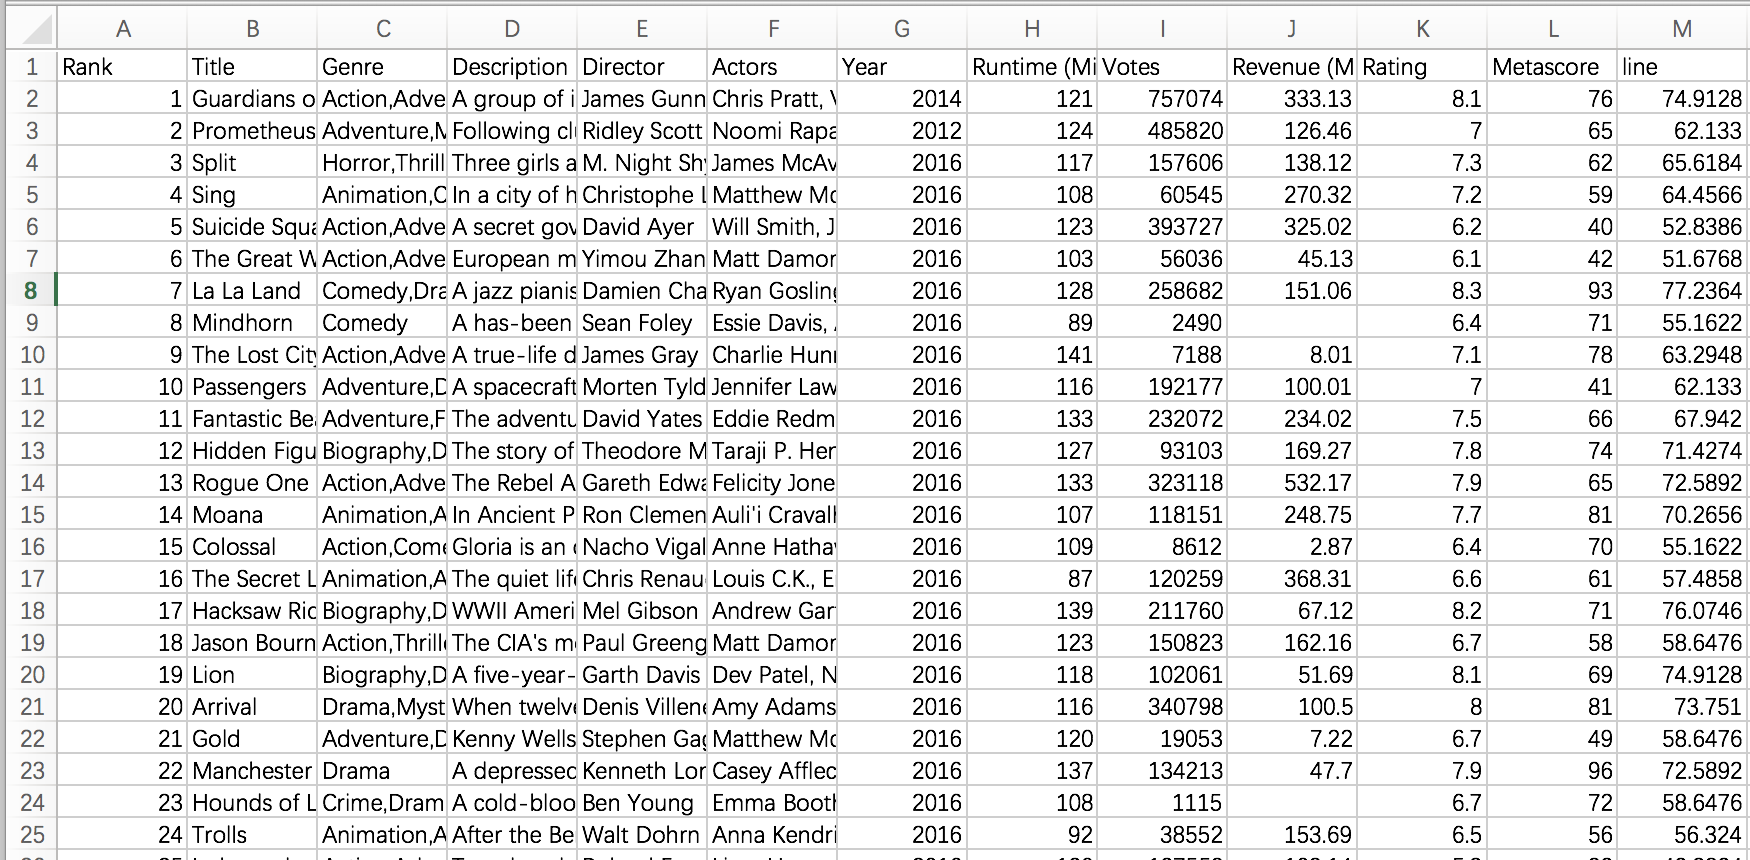
\includegraphics{excel-table.png}
\\
Then, we remove the line with empty value of MetaScore because in this
case, we require the data of MetaScore. After remove, we get 936 valid
record.
\\
Then, we user the Excel internal function to draw the scatter diagram of
the data and draw the line of \textbf{linear regression}
\\
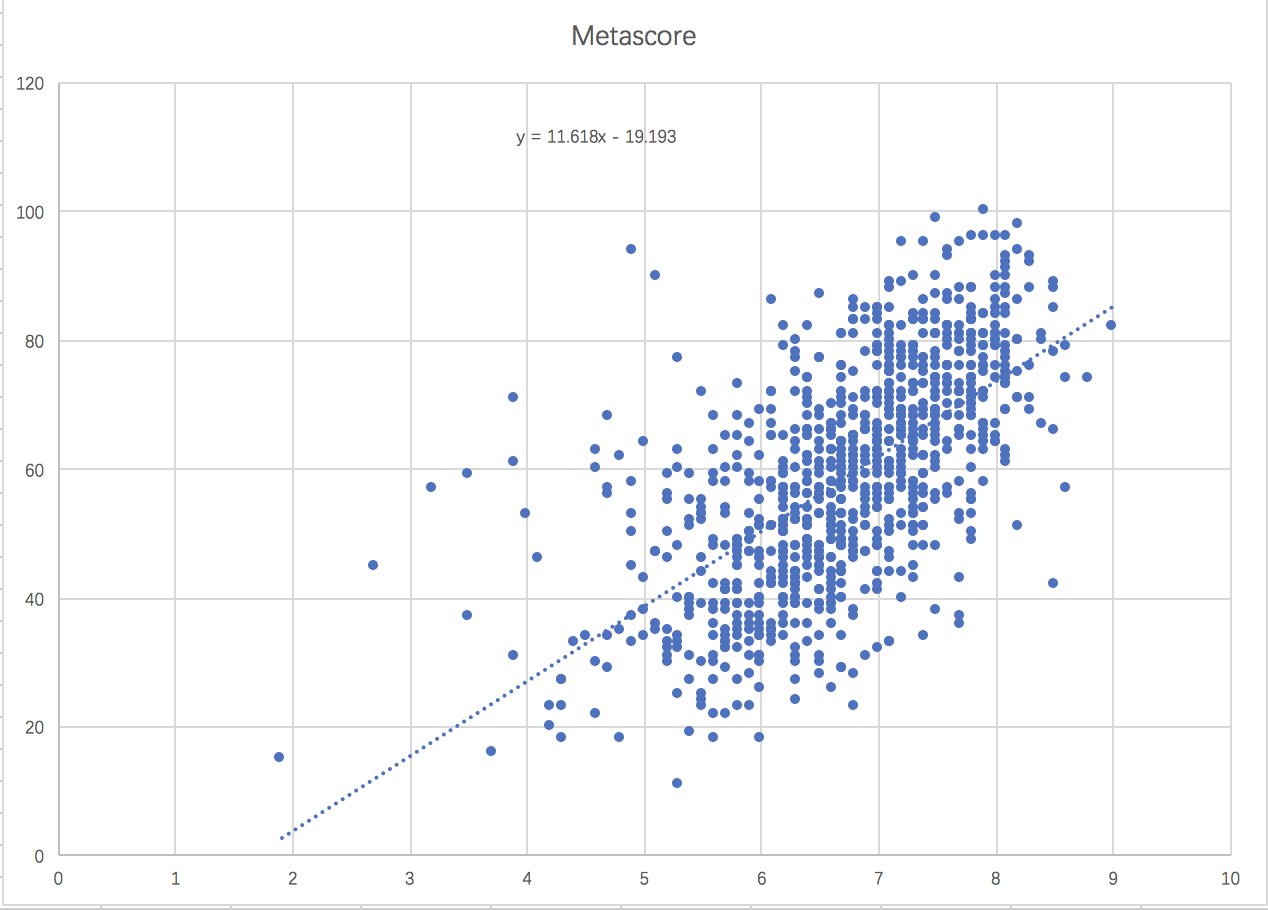
\includegraphics{linear-regreesion.png}
\\
The regression function is \texttt{y\ =\ 11.618x\ –\ 19.193}, where x is
rating and y is metascore.
\\
We calculate the absolute value between actual value and linear
regression and count the number of record.
\\
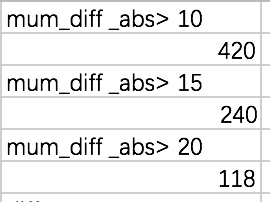
\includegraphics{abs-value.png}
\\
We assume that the top 5\% and lowest 5\% as the outlier.
\\
So, we need to get about 10\% of data: 20 is a suitable different.
\\
We first analysis the top 5\% (different \textgreater{}20) of the data,
which mean ``Low Rating but Has High MetaScore''. Then we can get: 
\\
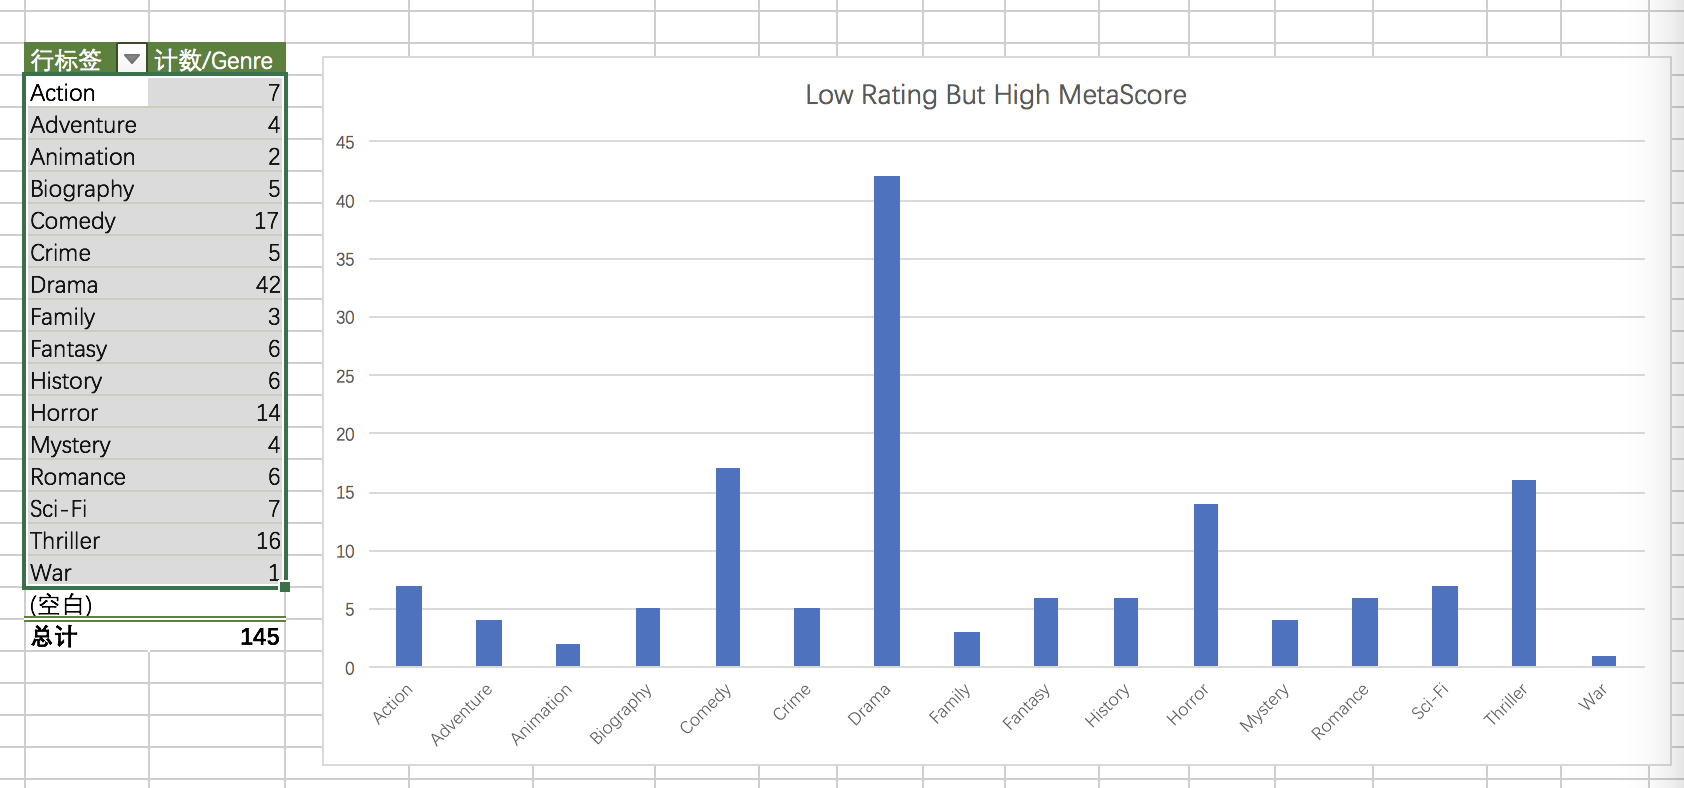
\includegraphics{5-precent.png}
\\
\textbf{We can clear know that Drama is the most common Genre in this
case.}
\\
Then, we analysis the lowest 5\% (different \textless{}-20) of the data,
which mean ``High Rating but Has Low MetaScore''. Then we can get:
\\
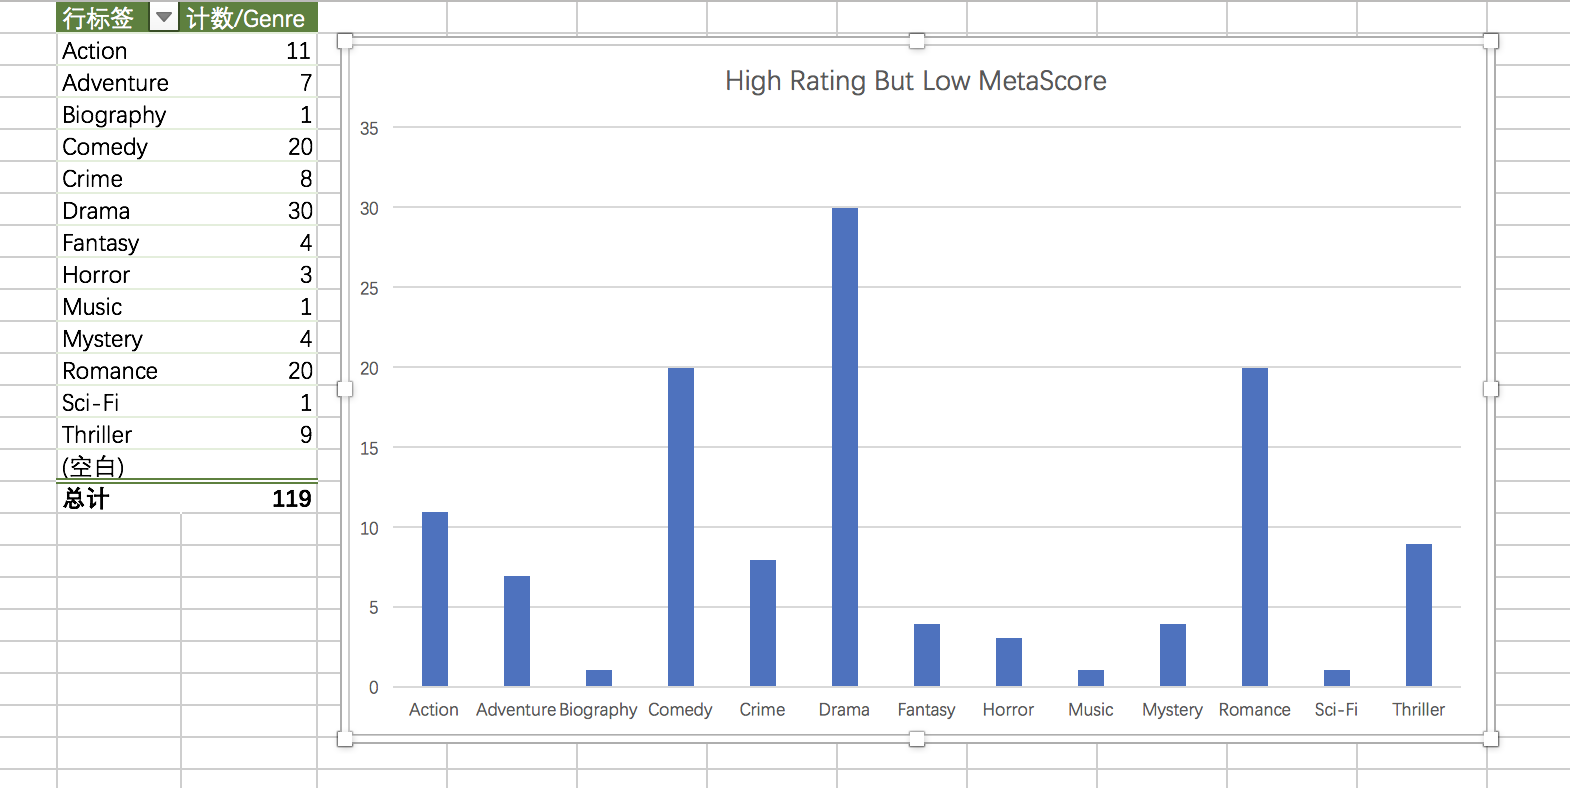
\includegraphics{high.png}
\\
\textbf{In this case, we also find that Drama is the most common Genre.}

    \subsubsection{Summary}\label{summary}

By analysis the result, we can conclude that Drama Movie has the most
controversial comment. Since it has the most gap between Rating and
MetaScore. It means the evaluation of Drama Movie is various among
people.
\\
For Drama movie, we should carefully consider the Rating and MetaScore,
because it has the most possibility that is a stray value.

    \subsection{Keywords Analyzing}\label{keywords-analyzing}

This analysis provided by Jiaqi (Garfield) Wu. By using these data, we
can create a word cloud based on the descriptions and to find out the
most frequent appeared keyword, and find out why the resulting words are
appeared so frequently.

\subsubsection{Implementation}\label{implementation}

\paragraph{Get the keywords}\label{get-the-keywords}

    \begin{Verbatim}[commandchars=\\\{\}]
{\color{incolor}In [{\color{incolor}4}]:} \PY{k+kn}{import} \PY{n+nn}{numpy} \PY{k}{as} \PY{n+nn}{np}
        \PY{k+kn}{import} \PY{n+nn}{pandas} \PY{k}{as} \PY{n+nn}{pd}
        \PY{k+kn}{import} \PY{n+nn}{matplotlib}\PY{n+nn}{.}\PY{n+nn}{pyplot} \PY{k}{as} \PY{n+nn}{plt}
        \PY{o}{\PYZpc{}}\PY{k}{matplotlib} inline
        \PY{k+kn}{import} \PY{n+nn}{seaborn} \PY{k}{as} \PY{n+nn}{sns}
        \PY{k+kn}{from} \PY{n+nn}{os} \PY{k}{import} \PY{n}{path}
        \PY{k+kn}{import} \PY{n+nn}{matplotlib}\PY{n+nn}{.}\PY{n+nn}{pyplot} \PY{k}{as} \PY{n+nn}{plt}
        \PY{k+kn}{import} \PY{n+nn}{random}
        \PY{k+kn}{from} \PY{n+nn}{wordcloud} \PY{k}{import} \PY{n}{WordCloud}\PY{p}{,} \PY{n}{STOPWORDS}
        \PY{n}{imdbdata}\PY{o}{=}\PY{n}{pd}\PY{o}{.}\PY{n}{read\PYZus{}csv}\PY{p}{(}\PY{l+s+s1}{\PYZsq{}}\PY{l+s+s1}{../Dataset/IMDB\PYZhy{}Movie\PYZhy{}Data.csv}\PY{l+s+s1}{\PYZsq{}}\PY{p}{)}
        \PY{n}{text} \PY{o}{=} \PY{p}{(}\PY{n+nb}{str}\PY{p}{(}\PY{n}{imdbdata}\PY{p}{[}\PY{l+s+s1}{\PYZsq{}}\PY{l+s+s1}{Description}\PY{l+s+s1}{\PYZsq{}}\PY{p}{]}\PY{p}{)}\PY{p}{)}
        \PY{n}{plt}\PY{o}{.}\PY{n}{subplots}\PY{p}{(}\PY{n}{figsize}\PY{o}{=}\PY{p}{(}\PY{l+m+mi}{20}\PY{p}{,}\PY{l+m+mi}{15}\PY{p}{)}\PY{p}{)}
        \PY{n}{wordcloud} \PY{o}{=} \PY{n}{WordCloud}\PY{p}{(}
                                  \PY{n}{stopwords}\PY{o}{=}\PY{n}{STOPWORDS}\PY{p}{,}
                                  \PY{n}{background\PYZus{}color}\PY{o}{=}\PY{l+s+s1}{\PYZsq{}}\PY{l+s+s1}{white}\PY{l+s+s1}{\PYZsq{}}\PY{p}{,}
                                  \PY{n}{width}\PY{o}{=}\PY{l+m+mi}{1500}\PY{p}{,}
                                  \PY{n}{height}\PY{o}{=}\PY{l+m+mi}{1200}
                                 \PY{p}{)}\PY{o}{.}\PY{n}{generate}\PY{p}{(}\PY{n}{text}\PY{p}{)}
        
        
        \PY{n}{plt}\PY{o}{.}\PY{n}{imshow}\PY{p}{(}\PY{n}{wordcloud}\PY{p}{)}
        \PY{n}{plt}\PY{o}{.}\PY{n}{title}\PY{p}{(}\PY{l+s+s1}{\PYZsq{}}\PY{l+s+s1}{Title}\PY{l+s+s1}{\PYZsq{}}\PY{p}{)}
        \PY{n}{plt}\PY{o}{.}\PY{n}{axis}\PY{p}{(}\PY{l+s+s1}{\PYZsq{}}\PY{l+s+s1}{off}\PY{l+s+s1}{\PYZsq{}}\PY{p}{)}
        \PY{n}{plt}\PY{o}{.}\PY{n}{show}\PY{p}{(}\PY{p}{)}
\end{Verbatim}


    \begin{center}
    \adjustimage{max size={0.9\linewidth}{0.9\paperheight}}{output_51_0.png}
    \end{center}
    { \hspace*{\fill} \\}
    
    \subsubsection{Summary}\label{summary}

From the graph, we can get these following keywords:
\begin{itemize}
    \item Year
    \item American
    \item Old
    \item Young
    \item Girl
\end{itemize}
Since most of the 1000 movies are American made, it is not surprising
that American will be one of the biggest word in the word cloud. It is
interesting that the word "girl" is much bigger than "boy". It shows
that people are more interesed in female rather than male. As for the
word "year", the reason of why it is so big is that when describing a
story, the timeline is always important. So the word "year" appeared
frequently in the describtion of movies.

\begin{center}
    \textbf{*** This is the end of the report. ***}
\end{center}
    
    \end{document}
